%%%%%%%%%%%%%%%%%%%%%%%%%%%%%%%%%%%%%%%%%%%%%%%%%%%%%%%%%%%%%%%%%%%%%%%%%%%%%%%%%%%%%%%%%%%%%%%
%%%%%%%%%%%%%%%%%%%%%%%%%%%%%%%%%%%%%%%%%%%%%%%%%%%%%%%%%%%%%%%%%%%%%%%%%%%%%%%%%%%%%%%%%%%%%%%
\section{Experimental Setup}\label{sec:xp:setup}

[TODO]

%%%%%%%%%%%%%%%%%%%%%%%%%%%%%%%%%%%%%%%%%%%%%%%%%%%%%%%%%%%%%%%%%%%%%%%%%%%%%%%%%%%%%%%%%%%%%%%
\subsection{Experimental Datasets}\label{sec:xp:data}

\begin{table*}[ht!]
\caption{Description of our six experimental datasets.}\label{tbl:dataset}
\begin{tabular}{m{2.2cm} m{5.4cm} m{7.4cm}}
\toprule
Dataset name & Samples & Description \\
\midrule

COIL20
    & 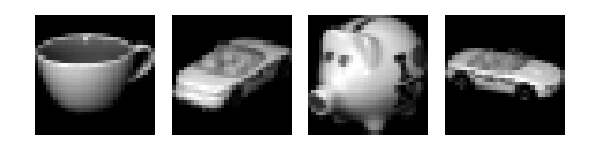
\includegraphics[width=\linewidth]{COIL20_samples}
    & 1440 gray-scale images of size 32x32, belonging to 20 classes.
    The raw images of 1024 dimensions are used directly for the DR methods.\\

DIGITS
    & 
\includegraphics[width=\linewidth]{DIGITS_samples}
    & 1797 gray-scale images of size 8x8 of 10 digits.
    The raw images of 64 dimensions are used directly for the DR methods.\\

{FASHION\_1K}
    & 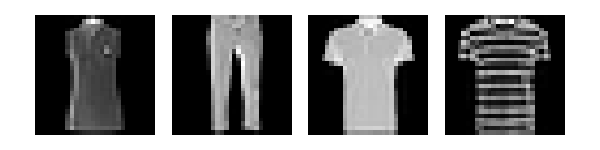
\includegraphics[width=\linewidth]{FASHION1000_samples}
    & 1000 gray-scale images of size 28x28 of 10 classes, sampled from Fashion-MNIST dataset.
    The raw images of 768 dimensions are used directly for the DR methods.\\

{FASH\_MOBI}
    & 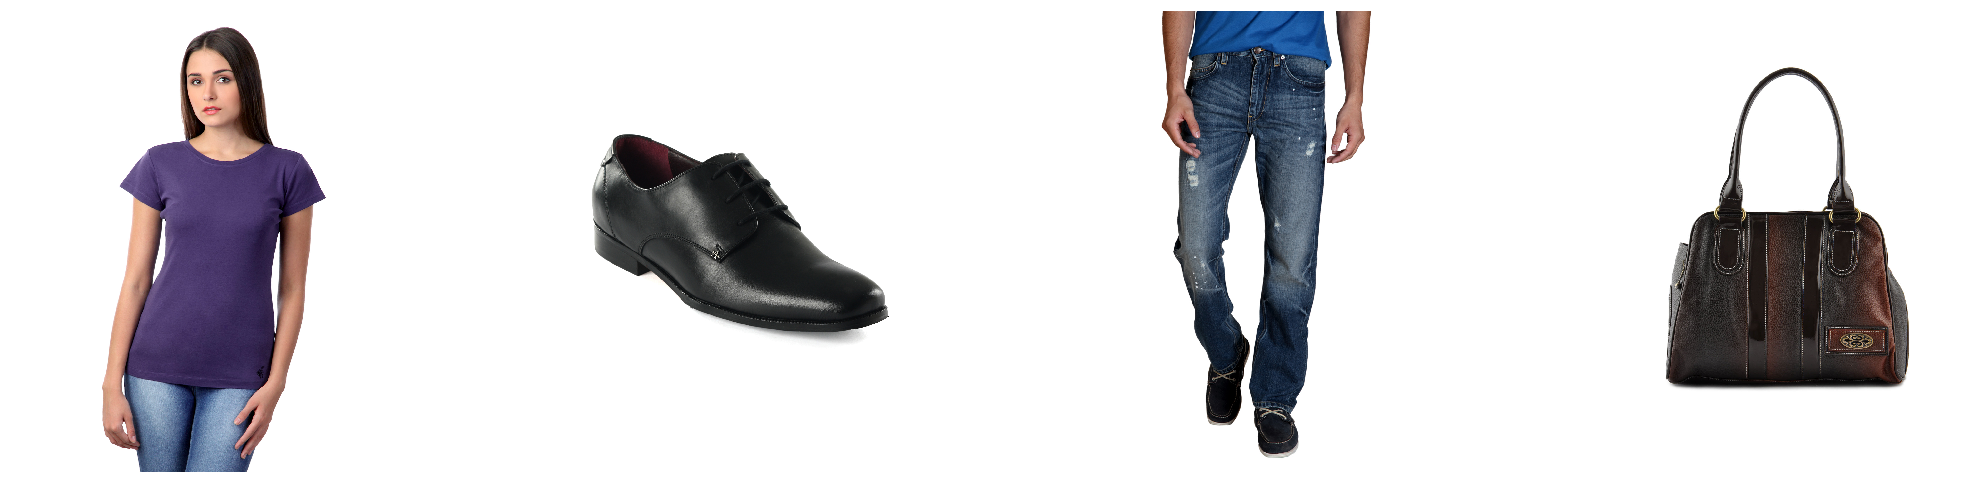
\includegraphics[width=\linewidth]{FASHION_PRODUCT_samples}
    & 1494 color images of various sizes belonging to 7 classes
    (\emph{'Bags', 'Bottomwear', 'Jewellery', 'Sandal', 'Shoes', 'Topwear', 'Watches'}),
    sampled from Fashion Product images dataset.\\

5NEWS
    & 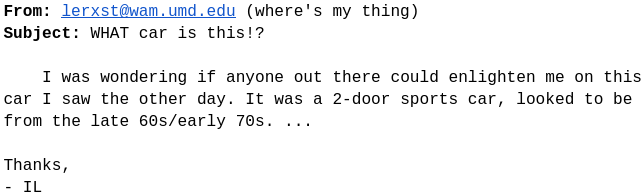
\includegraphics[width=\linewidth]{20NEWS5_samples}
    & 5 groups of 2957 emails selected from 20Newsgroups dataset,
    including \emph{'rec.autos', 'rec.sport.baseball','sci.crypt', 'sci.space', 'comp.sys.mac.hardware'}. \\

{NEURON\_1K}
    &
    & 1301 brain cells from a combined cortex, hippo-campus and sub-ventricular zone of an E18 mouse. \\

\bottomrule
\end{tabular}
\end{table*}

Six datasets of gray-scale and color images, text and gene expressions are used to demonstrate the application of our method (see Table~\ref{tbl:dataset} for examples of instances for each dataset).

A first baseline dataset, DIGITS, is a subset of the optical recognition of handwritten digits dataset of 8x8 gray-scale images \cite{kaynak1995methods}.
The second baseline dataset, COIL20, is a dataset of 32x32 gray-scale images of 20 rotated objects  \cite{nene1996}.
The third baseline dataset, {FASHION\_1K}, contains 1000 gray-scale images of size 28x28, sampled from Fashion-MNIST clothing dataset~\cite{xiao2017/online}.
The gray-scale images from the three above datasets are normalized and used directly in the DR methods.

Our first real-world image dataset, \emph{FASHION\_MOBILENET} dataset ({FASH\_MOBI} for short), contains samples of the seven most numerous classes from the fashion product images dataset~\cite{fashionproduct}.
The MobileNet\cite{howard2017mobilenets} with pre-trained weights from ImageNet is used for feature extraction, a transfer learning technique that uses the representation of the learned network (trained on a large-scale image classification task) to extract meaningful features for new samples.
The last fully connected layer of the network is replaced by a global average pooling layer \cite{lin2013network} to obtain the flattened output vector of 1280 dimensions.
To speed up DR methods for visualization task, PCA is then applied to take only 75 features.

The second real-word dataset is a textual dataset. The 5NEWS dataset contains the text of 5 groups selected from the 20 Newsgroups dataset, which are converted to a matrix of token counts via Term Frequency Inverse Document Frequency (TF-IDF) method.
The count vectors are then fed into a Latent Dirichlet Allocation (LDA)~\cite{blei2003latent} model to extract 15 hidden topics, which are the 15 features used by the DR methods.

Our last real-world dataset is the open {NEURON\_1K} dataset~\cite{neuron1k}, which contains 1301 brain cells from an E18 mouse. These cells have been processed and provided by 10X Genomics, a company who provides chromium single cell gene expression solution and releases several public genetic datasets.\footnote{https://www.10xgenomics.com/resources/datasets/, the datasets are licensed under the Creative Commons Attribution license.}
The processed data have 10 PCA features and 6 labels found by a graph-based clustering method.


%%%%%%%%%%%%%%%%%%%%%%%%%%%%%%%%%%%%%%%%%%%%%%%%%%%%%%%%%%%%%%%%%%%%%%%%%%%%%%%%%%%%%%%%%%%%%%%
\subsection{Constraint Generation}\label{sec:xp:constraint}

The input for our constraint preserving scores is an ensemble of constraints in the form of similar and dissimilar links.
% When labels are provided, they can be used to generate constraints. However, our method does not need many constraints to be stable, which means that we use a small subset of labeled instances to generate the constraints.
However, it is hard to control the quality of the constraints when they are selected manually.
For example, a similar link between two different data points is not expected.
The number of constraints of each type also affects the stability of the score.
In order to correctly evaluate the score function, we do not use the pairwise constraints directly, but use a small subset of labeled data points to generate the constraints instead.

Given a dataset of $C$ classes, $k$ labeled instances are randomly considered for each class.
Suppose that the number of instances in each class is larger than $k$ ($k$ is usually very small),
a similar link is formed by choosing a random pair of instances of each class.
This procedure leads to a number of similar links given by
\begin{equation}\label{eq:|S|}
    |\mathcal{S}| = C {k \choose 2} = \frac{1}{2} C k (k - 1).
\end{equation}

The dissimilar links are formed by first choosing two different classes among the $C$ classes (${C \choose 2}$ ways),
and then choosing a pair of two instances from these classes ($k^2$ pairs).
The number of all possible dissimilar links is therefore given by
\begin{equation}\label{eq:|D|}
    |\mathcal{D}| = {C \choose 2} k^2 = \frac{1}{2} C (C - 1) k^2.
\end{equation}

% This means that the more labeled instances are considered (i.e., $k$ is larger), the more constraints are generated and the more stable the $f_{score}$ is.
% For instance, with 10 labeled points for each of the 10 classes of the DIGITS dataset, 450 similar links and 4500 dissimilar links can be generated.
The labeled points are used to indicate the relationship of belonging to the same or to different groups.
The points can also be freely chosen and grouped by the users to indicate the relationship that they care about.
Intuitively, the generated pairwise constraints can express the information encoded in the labeled points.
$f_{score}$ function which takes the constraints as input will evaluate how well the encoded information is preserved in the embeddings.
The experimental setup for proving empirically the reliability of $f_{score}$ is presented in the next section.

%%%%%%%%%%%%%%%%%%%%%%%%%%%%%%%%%%%%%%%%%%%%%%%%%%%%%%%%%%%%%%%%%%%%%%%%%%%%%%%%%%%%%%%%%%%%%%%
\subsection{Score Preparation and Use of BayOpt in the Experiments}\label{sec:xp:proof}

% The experiments are designed to prove that $f_{score}$ provides good visualizations (Section~\ref{sec:result:bo}), as well as to prove its stability (Section~\ref{sec:result:stability}) and its flexibility (Section~\ref{sec:result:flexibility}).

A grid of hyperparameters for each of the three methods ($t$-SNE, LargeVis and UMAP) is created in order to evaluate $f_{score}$ for the embedding corresponding to each combination of their hyperparameters.
% In order to compute $f_{score}$ for each embedding corresponding to each combination of the hyperparameters, a grid of hyperparameters for each of the three methods ($t$-SNE, LargeVis and UMAP) is used.
In the case of $t$-SNE and LargeVis, the grid is an integer vector of perplexity values in $[2,N/3]$.
% , in which $N$ is the number of instances of the dataset.
% In the case of UMAP, the two dimensional grid contains combinations of its two hyperparameters.
% The first dimension is an integer vector of {n\_neighbor} values from 2 to $N/3$ in log-scale.
% The second dimension is a vector of 10 real values of {min\_dist} from 0.001 to 1.0 in log-scale.
% The grid is used to evaluate the reliability of the BayOpt approach on the proposed score.
In the case of UMAP, the two dimensional grid is created from an integer vector of {n\_neighbor} values in $[2,N/3]$ and a vector of 10 real values of {min\_dist} in $[0.001, 1.0]$.
All the hyperparameter values are sampled in natural logarithmic scale (log-scale) in order to focus the computation on the not-so-large hyperparameter values.
Finding the best hyperparameters by greedily searching through the grid is not practical and scalable.
BayOpt approach solves this scalability problem efficiently, in which only dozens of evaluations are required to find the best hyperparameters for all experimented datasets.

For the hyperparameter tuning task under BayOpt framework in this work, the exploration strategy is preferred to ensure to discover the largest as possible the parameter space.
% Three technical points that guarantees the accuracy in predicting the best hyperparameters and the quick convergence of BayOpt in our experiments are follows.
Expected Improvement (EI) acquisition function is used as a surrogate function of BayOpt.
In EI, the parameter $\xi$ controls the trade-off between global search (exploration) and local optimization (exploitation).
$\xi$ is set to a large value (0.1) to realized the exploration strategy, that works well for all experimented dataset without any effort to tune this parameter.
Since there is always a small variance in the score value, 
the input observations (the $f_{score}$ values) for BayOpt can be corrupted by noise.
Small values are added to the diagonal of the kernel function of the underlying Gaussian Process model in BayOpt to handle this noise.

%%%%%%%%%%%%%%%%%%%%%%%%%%%%%%%%%%%%%%%%%%%%%%%%%%%%%%%%%%%%%%%%%%%%%%%%%%%%%%%%%%%%%%%%%%%%%%%
%%%%%%%%%%%%%%%%%%%%%%%%%%%%%%%%%%%%%%%%%%%%%%%%%%%%%%%%%%%%%%%%%%%%%%%%%%%%%%%%%%%%%%%%%%%%%%%
\section{Experimental Results}\label{sec:results}

[TODO]

%%%%%%%%%%%%%%%%%%%%%%%%%%%%%%%%%%%%%%%%%%%%%%%%%%%%%%%%%%%%%%%%%%%%%%%%%%%%%%%%%%%%%%%%%%%%%%%
\subsection{$f_{score}$}\label{sec:result:fscore}
The behaviour of $f_{score}$ for the embeddings of three methods with all six experimented datasets is illustrated in Fig.~\ref{fig:score:all}.
The hyperparameter values are shown in logarithmic scale.
The score values for UMAP are shown for {min\_dist= 0.1}.
The contour plots of $f_{score}$ for all values of {min\_dist} are in Fig.~\ref{fig:score:umap2D:compare}.
The score values are calculated for a set of pairwise constraints generated from 10 labeled points per class for each dataset.
The pairwise constraints generated from these labeled points are sufficient to analyse the behaviour of $f_{score}$.   
For instance, with 10 labeled points for each of the 10 classes of DIGITS dataset, 450 similar links and 4500 dissimilar links can be generated.
The effect of the number of labeled points on $f_{score}$ will be evaluated in the next section.

%% FIGURE f_scores all datasets / all methods
\begin{figure*}[ht!]
    \centering
    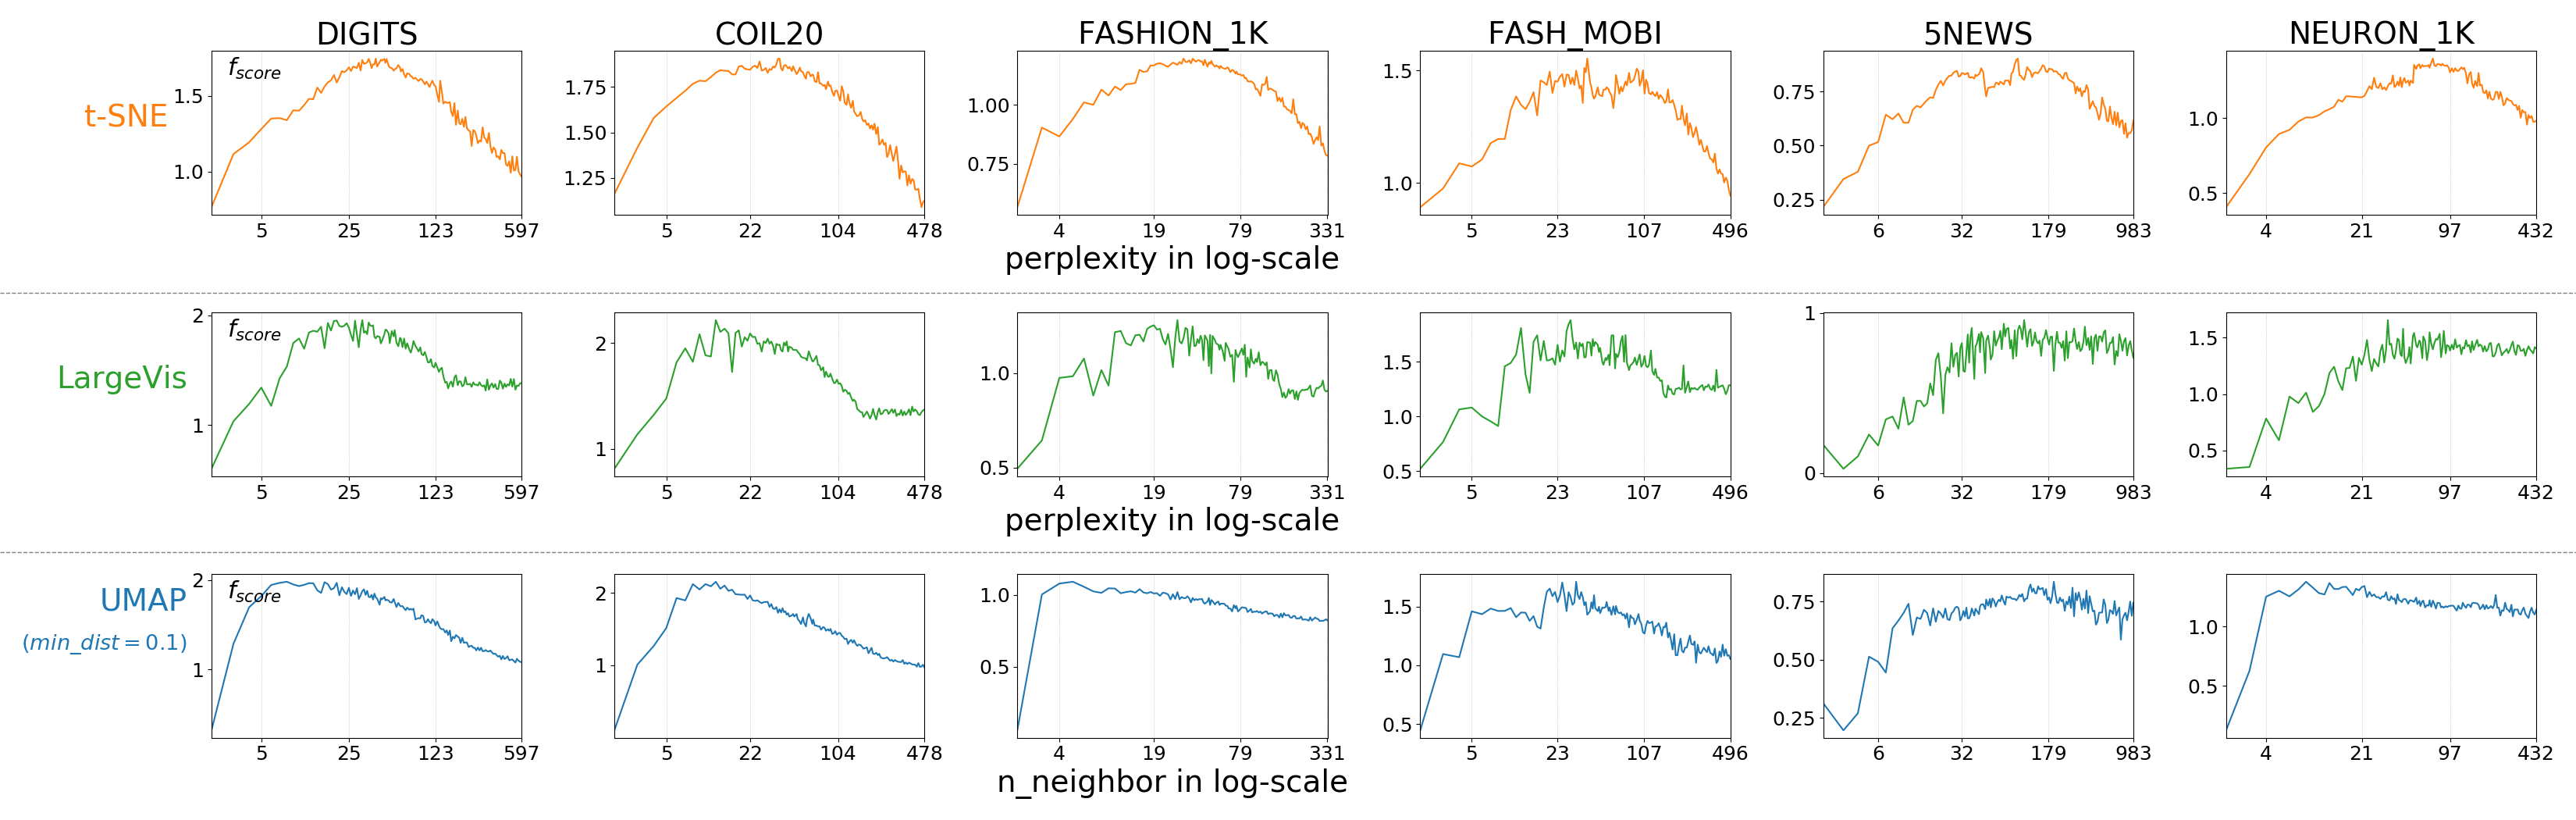
\includegraphics[width=\linewidth]{all_scores_all_methods}
    \caption{$f_{score}$ for all three methods for all six datasets.}
    \label{fig:score:all}
\end{figure*}

The key finding is that, $f_{score}$ has the form of a convex function: it increases when the number of neighbors (perplexity/{n\_neighbors}) increases, reaches its maximum value, and then decreases when the number of neighbors is too large.
The function of score values is not smooth as the input constraints vary,
% but all DR methods share this approximate convex form.
but it forms suggests that finding its global maximum is feasible.
In the case of LargeVis, there are flat regions where $f_{score}$ does not change too much.
The reason is that LargeVis is designed for large dataset and, thus, when applied to medium-sized datasets,
% a large set of perplexity values yield the same results.
the impact of perplexity is not important.
In contrast, $t$-SNE and UMAP are very sensitive to their hyperparameters.
Intuitively, when the number of neighbors is small, the points are not grouped in the visualization.
The similar links are unlikely preserved while the dissimilar links have more chance to be preserved as the points stay away from each other.
% In this case $f_{score}(\mathcal{S})$ is very low and $f_{score}(\mathcal{D})$ is high, that makes $f_{score}$ low.
Inversely, when the number of neighbors is large, every point is neighbor to each other, which make the visualization a big cluster.
In this case, the similar constraints are likely preserved while the dissimilar constraints are not.
% that make $f_{score}(\mathcal{S})$ high and $f_{score}(\mathcal{D})$ very low, and $f_{score}$ is low as a consequence.
Due to these trade-offs in both cases, $f_{score}$ in overall is always low. 

In summary, the local structures (neighborhood information) of a dataset are presented by the small groups in the visualization.
The clearer these groups are highlighted, the more likely the similar constraints of the points within groups and the dissimilar constraints of the points between different groups are preserved.
The proposed score has well captured this characteristic, it reaches to the high values only when both the similar and dissimilar constraints are preserved.
Thus $f_{score}$ can be used to quantitatively evaluate the quality of the visualization and can be comparable to the state of the art quality metrics.

%%%%%%%%%%%%%%%%%%%%%%%%%%%%%%%%%%%%%%%%%%%%%%%%%%%%%%%%%%%%%%%%%%%%%%%%%%%%%%%%%%%%%%%%%%%%%%%
\subsection{Stability of $f_{score}$}\label{sec:result:stability}

%% FIGURE score stability
\begin{figure}[ht!]
\begin{subfigure}[b]{0.32\linewidth}
     \centering
     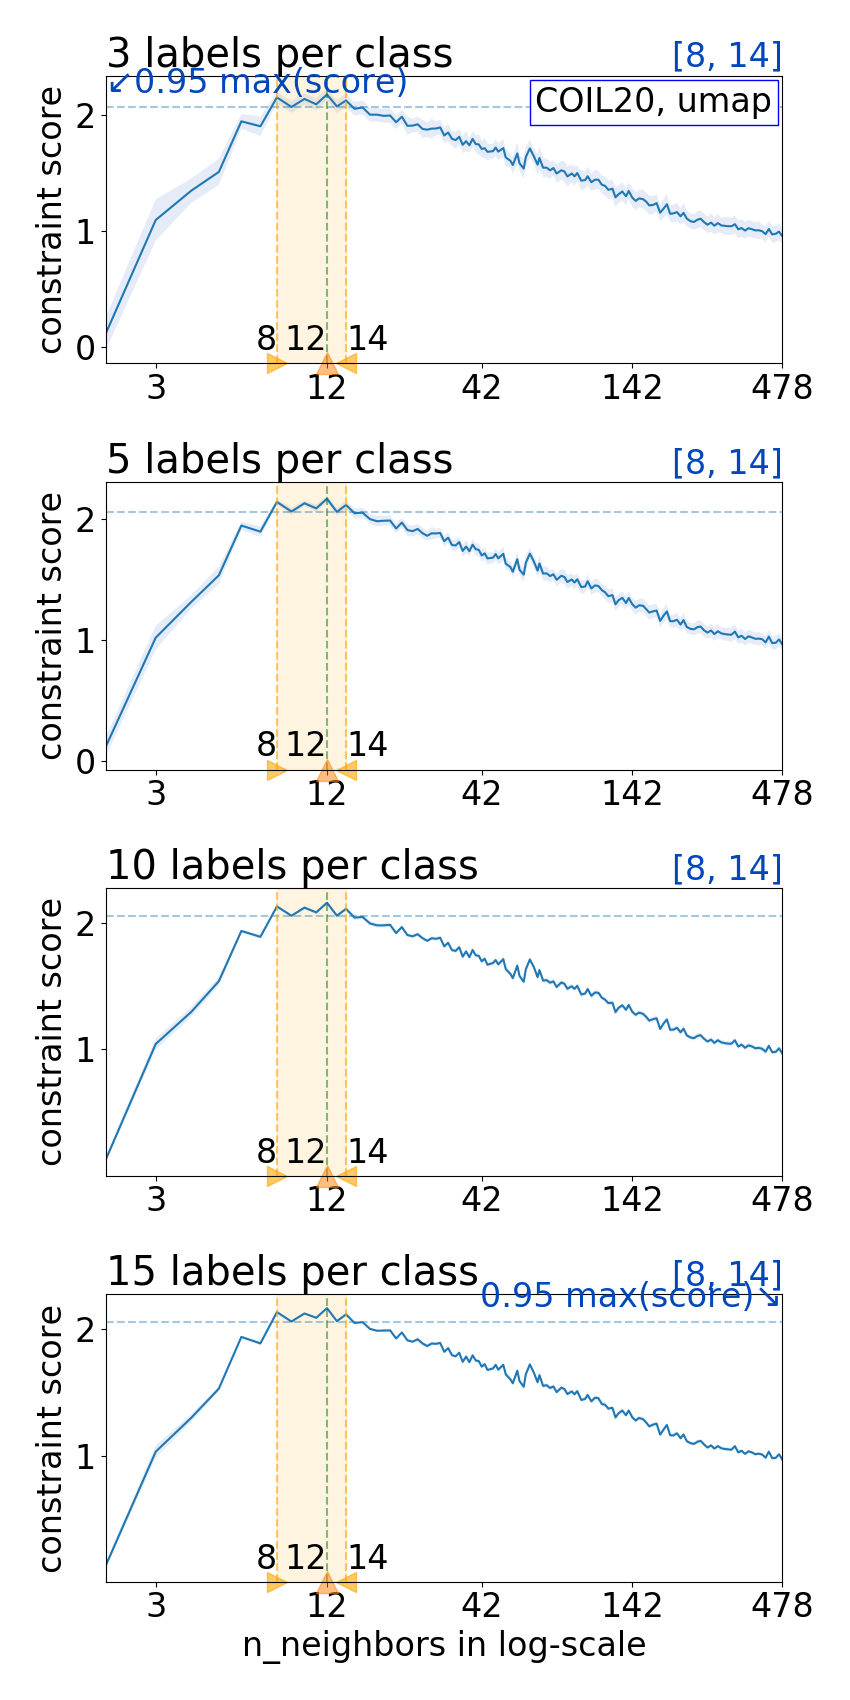
\includegraphics[width=\linewidth]{COIL20_umap_scores}
     \caption{UMAP}
\end{subfigure}
\hfill
\begin{subfigure}[b]{0.32\linewidth}
     \centering
     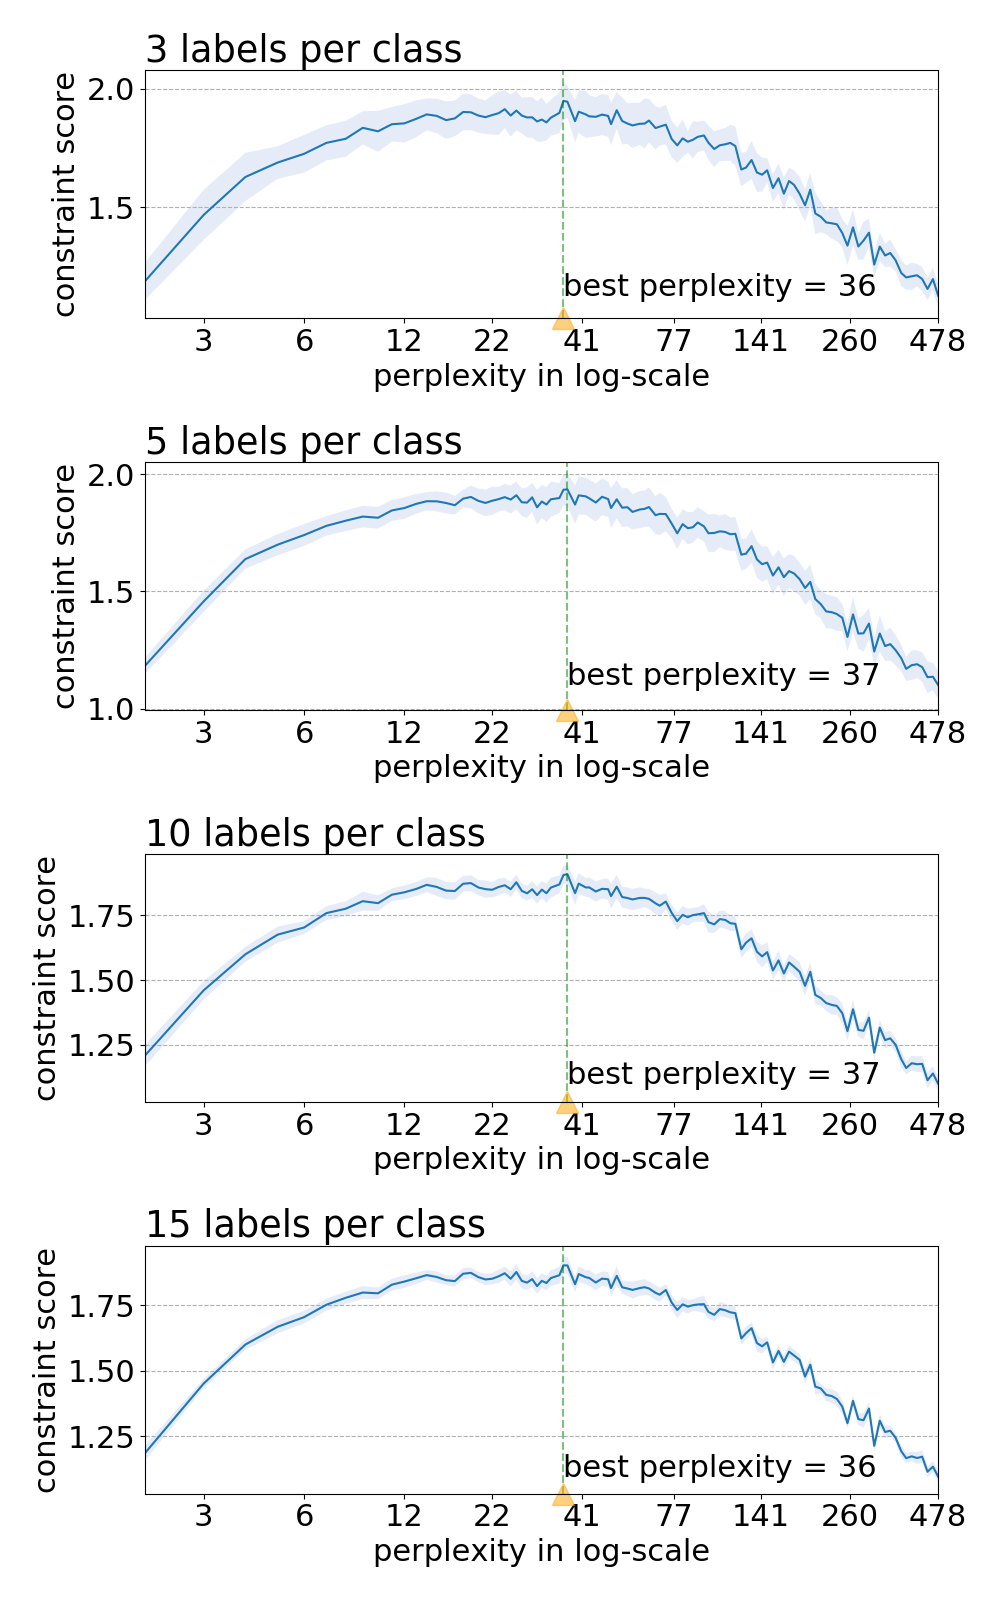
\includegraphics[width=\linewidth]{COIL20_tsne_scores}
     \caption{$t$-SNE}
\end{subfigure}
\hfill
\begin{subfigure}[b]{0.32\linewidth}
     \centering
     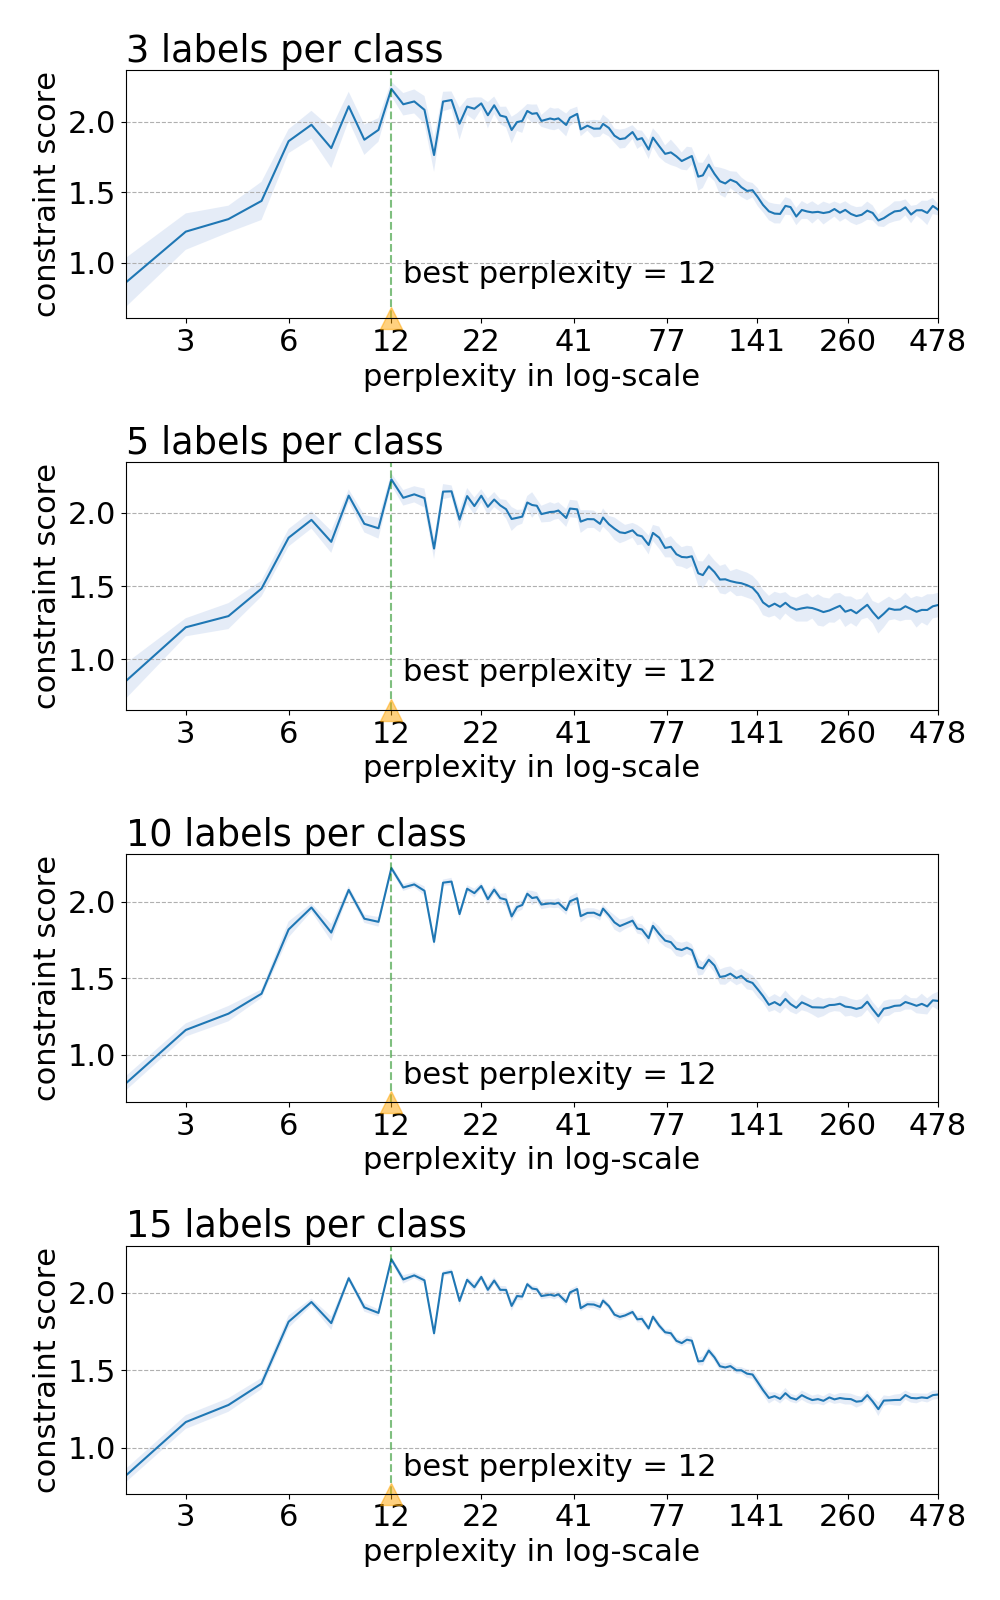
\includegraphics[width=\linewidth]{COIL20_largevis_scores}
     \caption{LargeVis}
\end{subfigure}
\caption{Stability of the constraint preserving scores with UMAP, $t$-SNE and LargeVis for COIL20 dataset.
The filled region highlights the best range of hyperparameters which make the score value superior to 96\% of maximum score value.}
\label{fig:score:stability:COIL20}
\end{figure}

The proposed constraint preserving score is a function of the pairwise constraints that may be generated automatically from input labels.
% In Eq.~\ref{eq:|S|} and Eq.~\ref{eq:|D|}, $k$ represents the number of instances that we consider for each given label.
% This $k$ is an hyperparameter of $f_{score}$.
% While it may be argued that the automatic tuning of DR hyperparameters is replaced by the manual tuning of the $f_{score}$ hyperparameter, this section shows that $f_{score}$ values are stable under changes of $k$.
% Another question that must be answered is whether if $f_{score}$ is stable for a fixed $k$, but with different constraints chosen given this $k$.
The more labeled points we have, the more constraints are generated, and as demonstrated as follows, the more stable the $f_{score}$ is.
The first question is, what is a reasonable small number of labeled points needed for each class to produce a stable $f_{score}$?
Moreover, with a fixed number of labeled points we can generate different set of pairwise constraints.
The second question is, with different set of constraints generated from the same fixed number of labeled points, is $f_{score}$ stable?
In order to answer these two questions, $f_{score}$ is evaluated for five different numbers of labeled points (3, 5, 10 and 15) per class.
The labeled points are independent and not accumulated.
This means that, for instance, the set of labeled points in the second setting does not contain the labeled points in the first setting.
In each setting for a fixed number of labeled points, the average value and the standard deviation of $f_{score}$ are analyzed w.r.t. 20 different sampled sets of pairwise constraints.

Fig.~\ref{fig:score:stability:COIL20} shows $f_{score}$ results for $t$-SNE, LargeVis and UMAP (with fixed {min\_dist} of 0.1) embeddings of COIL20 dataset.
The results are shown for COIL20, but are also true for the other selected datasets.
When the number of labeled instances increases, $f_{score}$ is more stable since the variance (presented by filled regions around the $f_{score}$ curve in Fig.~\ref{fig:score:stability:COIL20}) decreases.

Selecting the best hyperparameter values corresponding to the maximum score may not be the best choice, since several hyperparameter values can give almost the same $f_{score}$.
In order to tackle this problem, a range of hyperparameter values that has $f_{score}$ larger than a threshold is selected.
For instance, the threshold can be 96\% of the maximum $f_{score}$ value.
The best hyperparameter ranges highlighted by the vertical regions in Fig.~\ref{fig:score:stability:COIL20} are sensibly the same for the different numbers of labeled instances selected per label (3, 5, 10 and 15).
% Fig.~\ref{fig:score:stability:COIL20} demonstrates that the best hyperparameter value ranges are sensibly the same for the different numbers of labeled instances selected per label (3, 5, 10 and 15).

% In the case of LargeVis, there are flat regions where $f_{score}$ does not change too much.
% The reason for this behavior is that LargeVis is designed for large dataset and, thus, when applied to medium-sized datasets, a large set of perplexity values yield the same results.
% In contrast, $t$-SNE and UMAP are very sensitive to their hyperparameters.
% Intuitively, when the number of neighbors is small, the points are not grouped in the visualization.
% The similar links are unlikely preserved while the dissimilar links have more change to be preserved since the points stay away from each other.
% In this case $f_{score}(\mathcal{S})$ is very low and $f_{score}(\mathcal{D})$ is high, that makes $f_{score}$ low.
% Inversely, when the number of neighbors is large, every point is neighbor to each other, which make the visualization a big cluster.
% In this case, the similar constraints are likely preserved while the dissimilar constraints are not, that make $f_{score}(\mathcal{S})$ high and $f_{score}(\mathcal{D})$ very low, and $f_{score}$ is low as a consequence.

% In summary, the local structures (neighborhood information) of a dataset are presented by the small groups in the visualization.
% The clearer these groups are highlighted, the more likely the similar constraints of the points within groups and the dissimilar constraints of the points between different groups are preserved.
% The proposed score has well captured this characteristic, it reaches to the high values only when both the similar and dissimilar constraints are preserved.
% Thus $f_{score}$ can be used to quantitatively evaluate the quality of the visualization and can be comparable to the state of the art quality metrics.
In summary, for all selected datasets, the above results indicate that 10 labeled instances per class is enough for obtaining a stable score.
The generated constraints from labeled points can capture the class-based relationship (local structure) that is typically well revealed by all three examined DR methods.
In Sec.~\ref{sec:result:flexibility}, we show that $f_{score}$ with different sets of labeled instances, which does not necessarily correspond to class labels,
can be used to encode the users' desired structure in the data.
% can be used as prior knowledge to generate constraints.
% This advocate for the flexibility of $f_{score}$, as any form of prior knowledge that can be formulated by pairwise constraints can be used.


%%%%%%%%%%%%%%%%%%%%%%%%%%%%%%%%%%%%%%%%%%%%%%%%%%%%%%%%%%%%%%%%%%%%%%%%%%%%%%%%%%%%%%%%%%%%%%%
\subsection{Comparison between $f_{score}$, $AUC_{log}RNX$ and BIC-based score}\label{sec:result:bo}

The proposed $f_{score}$ is compared with $AUC_{log}RNX$ and BIC-based score in the task of evaluating $t$-SNE embeddings in Sec.~\ref{sec:compare:tnse}.
It is compared with $AUC_{log}RNX$ in the task of evaluating UMAP embeddings in Sec.~\ref{sec:compare:umap}.
In all comparison, $f_{score}$ is calculated from the constraints generated by 10 labeled points per class on each dataset.

\subsubsection{Compare $f_{score}$, $AUC_{log}RNX$ and BIC-based score for $t$-SNE embeddings}\label{sec:compare:tnse}

%% FIGURE metamap tSNE example
\begin{figure*}[ht!]
    \centering
    \begin{subfigure}[b]{.8\linewidth}
        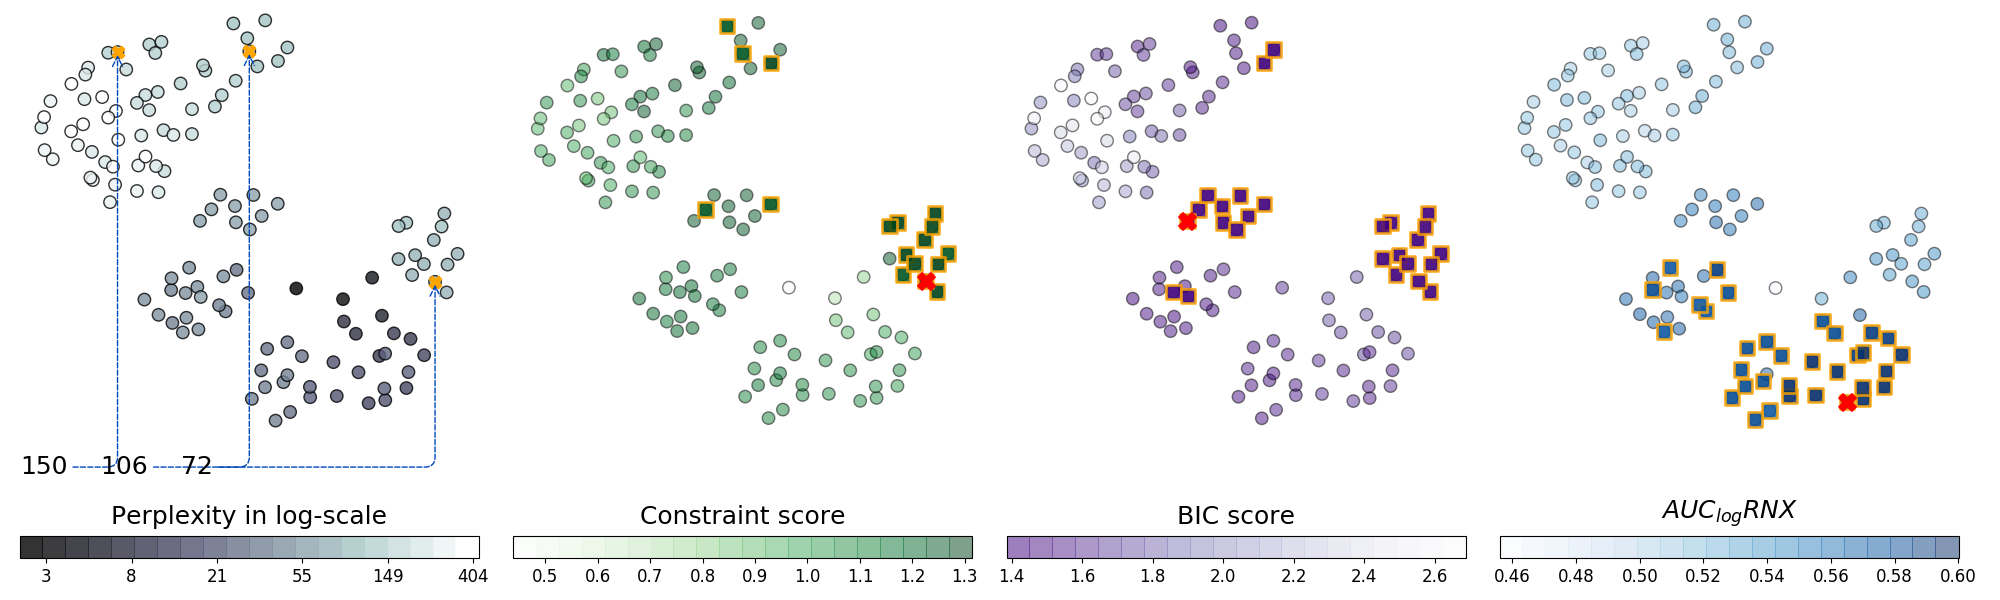
\includegraphics[width=\linewidth]{NEURON_1K_tsne_metamap}
    \end{subfigure}
    ~
    \begin{subfigure}[b]{.8\linewidth}
        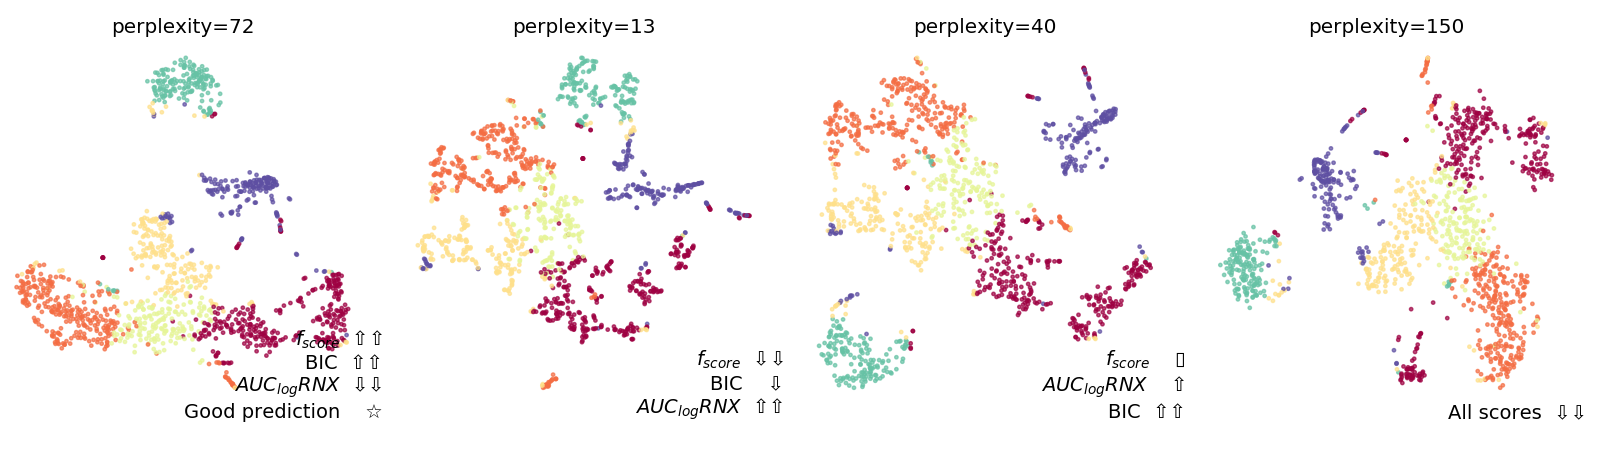
\includegraphics[width=\linewidth]{NEURON_1K_tsne_show}
    \end{subfigure}
    \caption{Metamap and sample visualizations for the selected parameters for {NEURON\_1K} dataset.}
    \label{fig:tsne:meta:NEURON1K}
\end{figure*}

%% FIGURE compare 3 scores tSNE
\begin{figure}[ht!]
    \centering
    \begin{subfigure}[b]{0.3\linewidth}
        \centering
        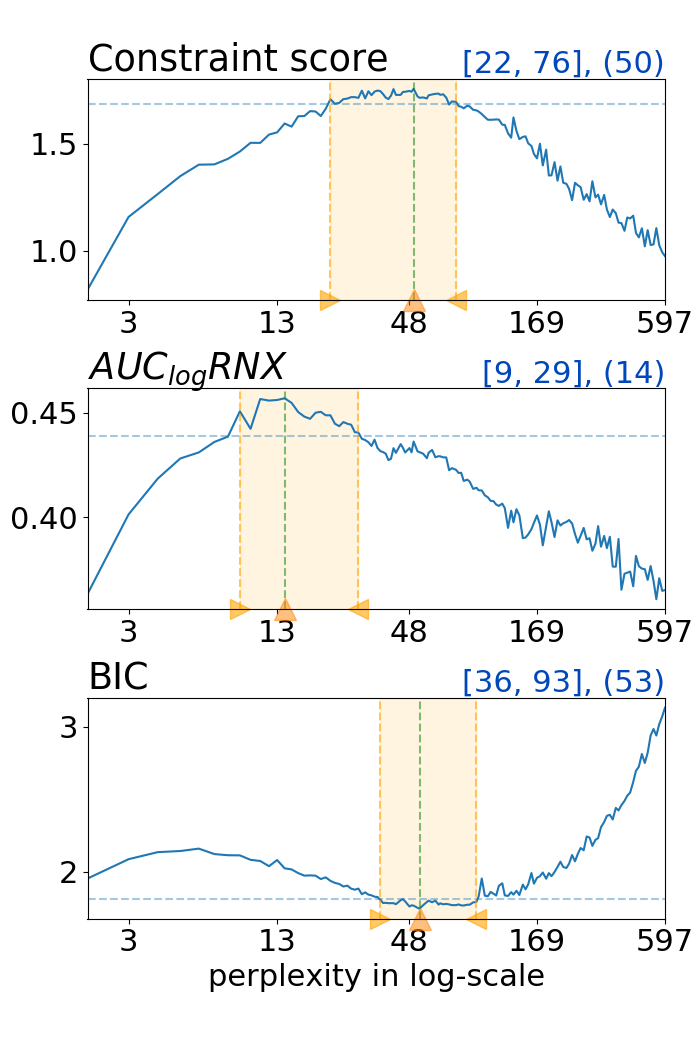
\includegraphics[width=\linewidth]{DIGITS_tsne_compare_scores}
        \caption{DIGITS}
    \end{subfigure}
    ~
    \begin{subfigure}[b]{0.3\linewidth}
        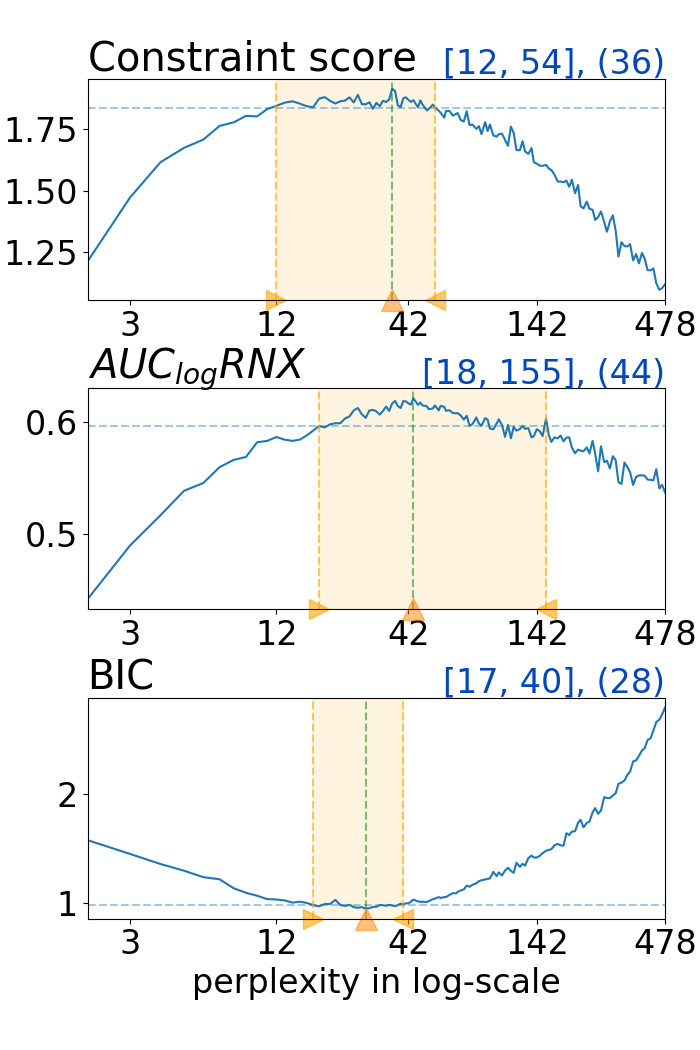
\includegraphics[width=\linewidth]{COIL20_tsne_compare_scores}
        \caption{COIL20}
    \end{subfigure}
    ~
    \begin{subfigure}[b]{0.3\linewidth}
        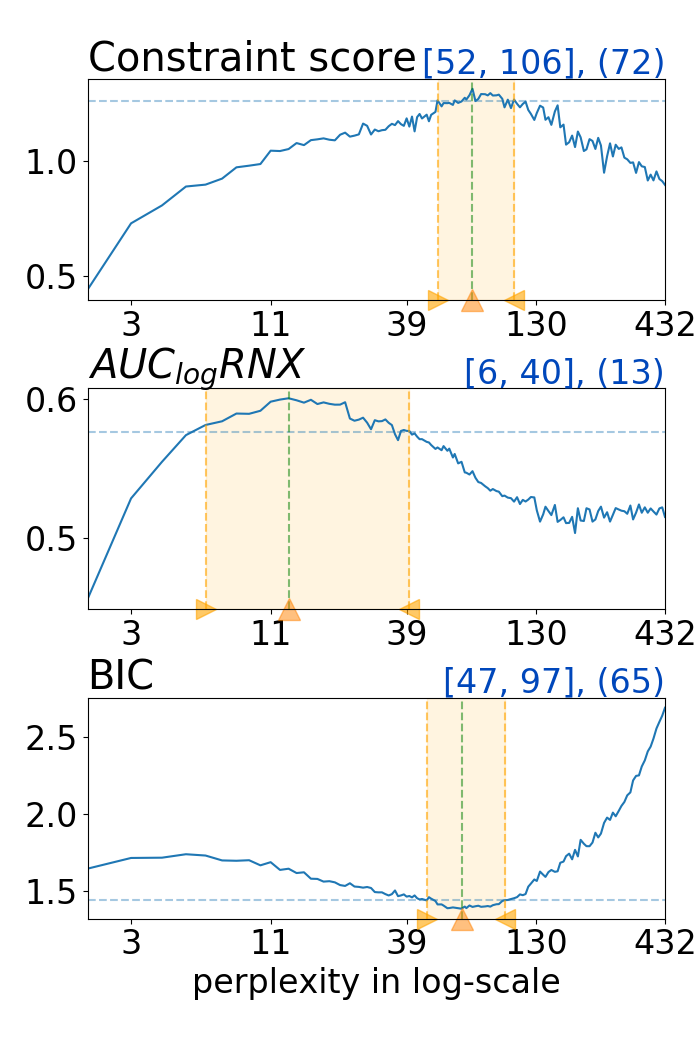
\includegraphics[width=\linewidth]{NEURON_1K_tsne_compare_scores}
        \caption{NEURON\_1K}
    \end{subfigure}
    \vfill
    \begin{subfigure}[b]{0.3\linewidth}
        \centering
        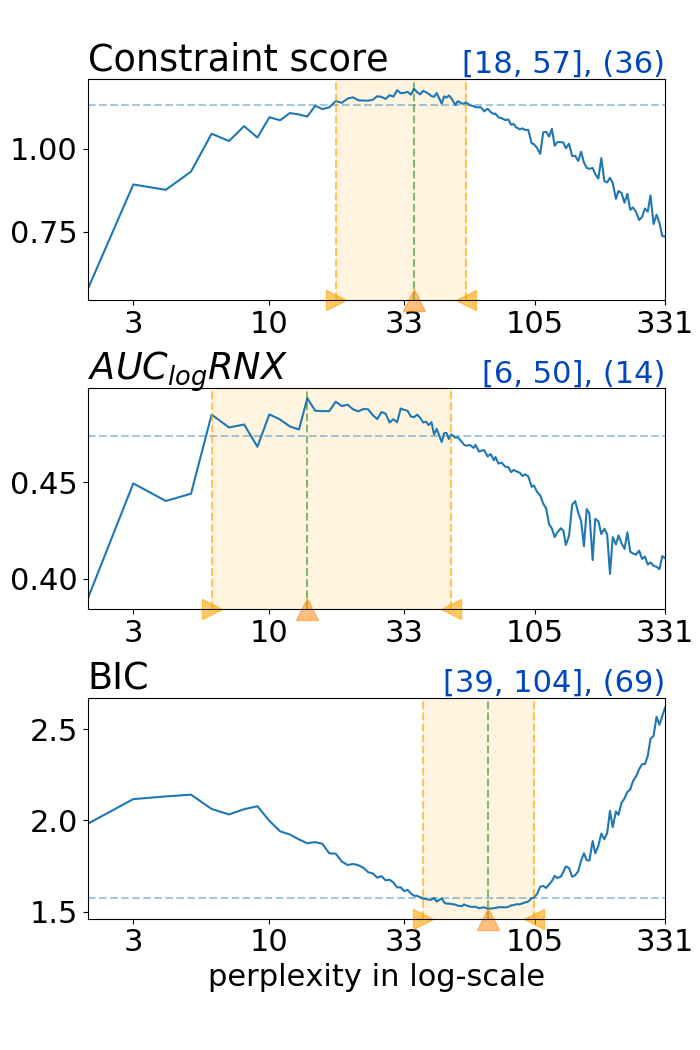
\includegraphics[width=\linewidth]{FASHION1000_tsne_compare_scores}
        \caption{FASHION\_1K}
    \end{subfigure}
    ~
    \begin{subfigure}[b]{0.3\linewidth}
        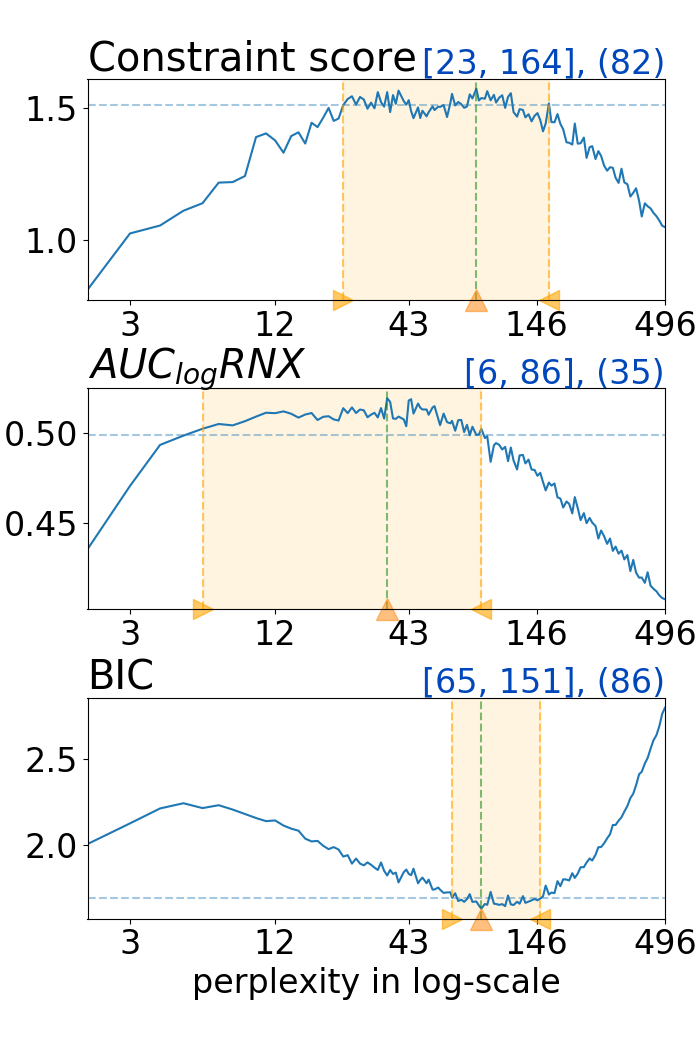
\includegraphics[width=\linewidth]{FASHION_MOBILENET_tsne_compare_scores}
        \caption{FASH\_MOBI}
    \end{subfigure}
    ~
    \begin{subfigure}[b]{0.3\linewidth}
        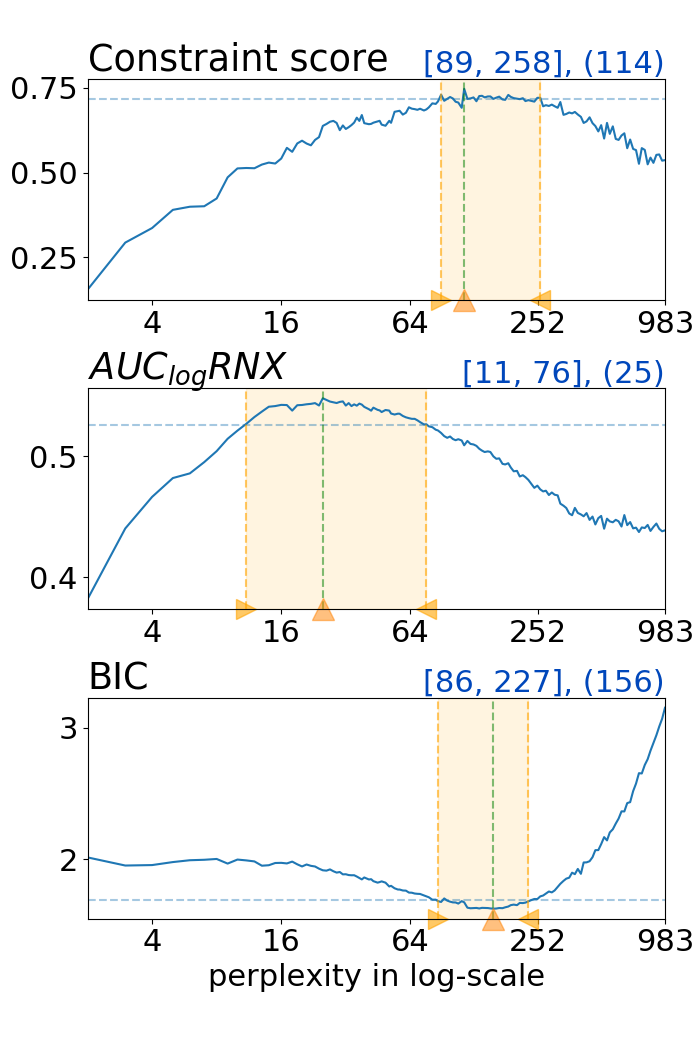
\includegraphics[width=\linewidth]{20NEWS5_tsne_compare_scores}
        \caption{5NEWS}
    \end{subfigure}
    \caption{Comparison of constraint score, $AUC_{log}RNX$ score and BIC score for $t$-SNE's embeddings.}
    \label{fig:tsne:compare}
\end{figure}

Fig.~\ref{fig:tsne:compare} illustrates the best perplexity range found by $f_{score}$, $AUC_{log}RNX$ and the BIC-based score for the six selected datasets.
$f_{score}$ agrees with both $AUC_{log}RNX$ and the BIC-based score for COIL20 and {FASH\_MOBI} datasets.
$f_{score}$ agrees only with $AUC_{log}RNX$, but not the BIC-based score for {FASHION\_1K} dataset.
Moreover, $f_{score}$ agrees only with the BIC-based score, but not $AUC_{log}RNX$, for {NEURON\_1K}, 5NEWS and DIGITS datasets.
In order to compare thoroughly the best solutions found by these three scores, metamaps can be used.

% Four metamaps for the {NEURON\_1K} dataset are presented in Fig.~\ref{fig:tsne:meta:NEURON1K}.
% Each metamap is used to visualize the solution space of a DR visualization, i.e., to represent embeddings with different perplexities on a 2D space.
A metamap is used to visualize the solution space of a DR visualization, i.e., to represent embeddings with different perplexities on a 2D space.
Each point in this metamap is an embedding corresponding to one perplexity, meaning that two points close together correspond to perplexities that provide similar visualizations.
The metamaps presented in this section contains points that are $t$-SNE visualizations, and are built by UMAP with {n\_neighbors} = 50 and {min\_dist} = 0.1.
UMAP with large {n\_neighbors} is used to build the metamap in order to obtain an overall view about the global relation of all embeddings.
% UMAP is used to build the metamap because of its capacity to consider the overall view, in addition to its focus on neighborhoods.
% Indeed, the large value of {n\_neighbors} (50) is used to obtain an overall view about the global relation of all embeddings.

In Fig.~\ref{fig:tsne:meta:NEURON1K}, some selected perplexity values are highlighted in the metamaps for {NEURON\_1K} dataset, and the corresponding visualizations are shown below them.
The four metamaps are colored by the values of perplexity, $f_{score}$, $AUC_{log}RNX$ and the BIC-based score respectively.
The embeddings with the highest score (superior than 96\% of maximum score) are highlighted.
For the real world {NEURON\_1K} dataset, the three scores discover different regions in the solution space. This can help the user to observe the structure of the dataset under different aspects given by the different quality scores.
% In ~\ref{app:tsne:meta}, an example where $f_{score}$ highly agrees with BIC-based score for DIGITS dataset is shown in Fig.~\ref{fig:app:tsne:meta:DIGITS}
% and an example where it agrees with both $AUC_{log}RNX$ and BIC-based score for {FASHION\_1K} datasets is shown in Fig.~\ref{fig:app:tsne:meta:FASHION1K}.

The visualizations at the bottom of Fig.~\ref{fig:tsne:meta:NEURON1K} served as a qualitative evaluation of the best visualizations found by $f_{score}$, $AUC_{log}RNX$ and the BIC-based score.
The ranks used for the scores are: very preferred ($\Uparrow\Uparrow$), preferred ($\Uparrow$), good enough ($[]$), not preferred ($\Downarrow$) and unfavorable ($\Downarrow\Downarrow$).
The visualization that is best predicted by BayOpt is denoted by a star symbol ($\star$).
As indicated by Wattenberg et. al.~\cite{wattenberg2016use}, more than one visualization may be needed to understand the high-dimensional patterns in the data.
The visualizations extracted thanks to the different scores make it easier to discover different regions in the solution space, and thus to discover different structures in the data, while one score could not reveal them all.

\subsubsection{Compare $f_{score}$ and $AUC_{log}RNX$ for UMAP embeddings}\label{sec:compare:umap}

A two dimensional grid of {n\_neighbors} and {min\_dist} hyperparameters are created to evaluate $f_{score}$ and $AUC_{log}RNX$ for the UMAP embeddings of all six datasets.
The values of these two scores are shown in the contour plots in Fig.~\ref{fig:score:umap2D:compare}.
{n\_neighbors} plays the same role as the perplexity of $t$-SNE and LargeVis.
It controls how large structures in the data should be conserved and affects the construction of the k-neighbor graph in HD.
A small value leads to many small connected components in the visualization, while a large value provides a boarder view of the data.
A suggested range for {n\_neighbors} is $[5, 50]$.
{min\_dist} in its turn, affects directly the output since it controls how tightly points are packed together. It is considered to be most important hyperparameter for UMAP \cite{mcinnes2018umap}.
The recommended range for {min\_dist} is $[0.001, 0.5]$.

For the three simple datasets (DIGITS, COIL20 and {FASHION\_1K}), $f_{score}$ shows clearly the evolution of the score value in comparison to $AUC_{log}RNX$.
For {NEURON\_1K} dataset, the two score discover different optimal zones but with the same principle.
For the two other datasets ({FASH\_MOBI} and 5NEWS), $AUC_{log}RNX$ shows clearer the zones of the best hyperparameters.
However, in general, the contour plots of $AUC_{log}RNX$ suggest that this score is not sensitive to the {min\_dist} hyperparameter.
Indeed, with a fixed value of {n\_neighbor}, it is likely that $AUC_{log}RNX$ gives the same score for different values of {min\_dist}.
In contrast, $f_{score}$ can discover the influence of {min\_dist} in conjunction with {n\_neighbor} in order to reveal the 

%% FIGURE metamap UMAP example
\begin{figure*}[ht!]
    \centering
    \begin{subfigure}[b]{.8\linewidth}
        \centering
        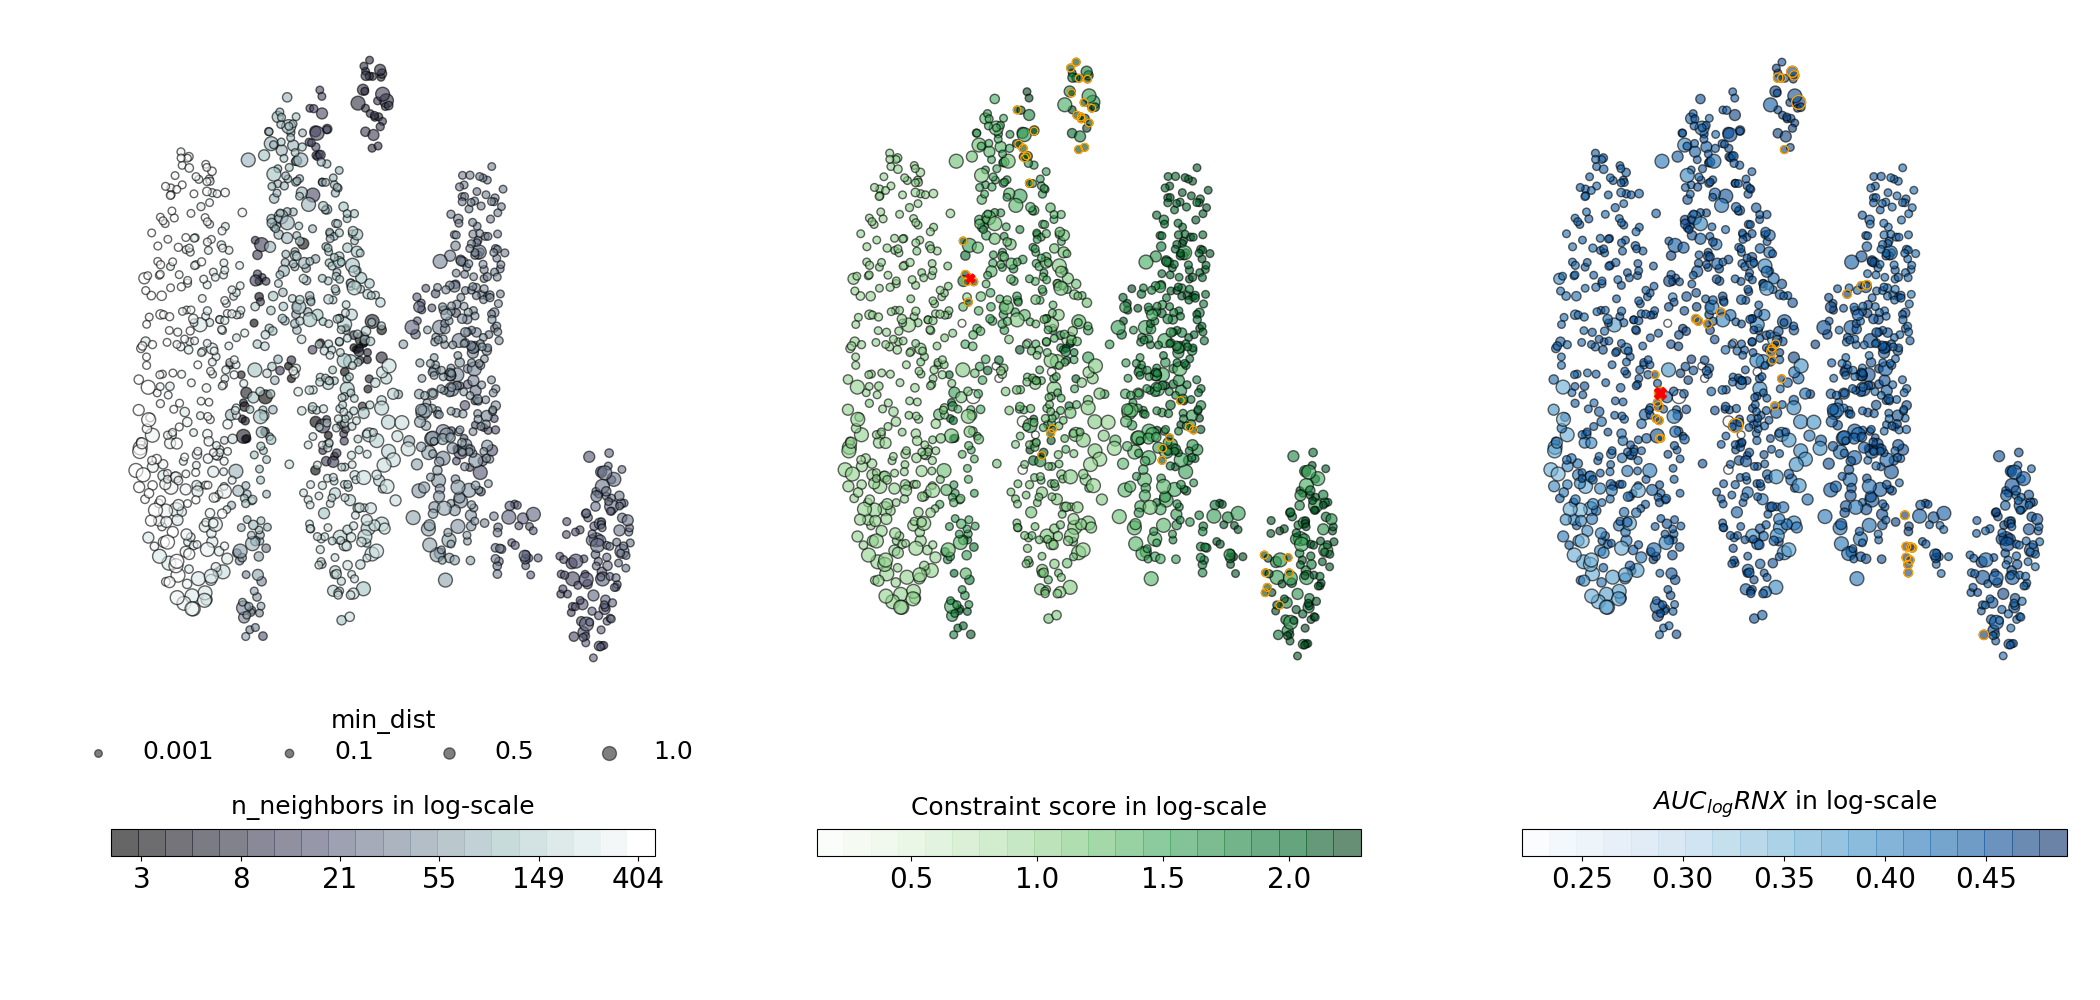
\includegraphics[width=\linewidth]{COIL20_umap_metamap}
    \end{subfigure}
    ~
    \begin{subfigure}[b]{.8\linewidth}
        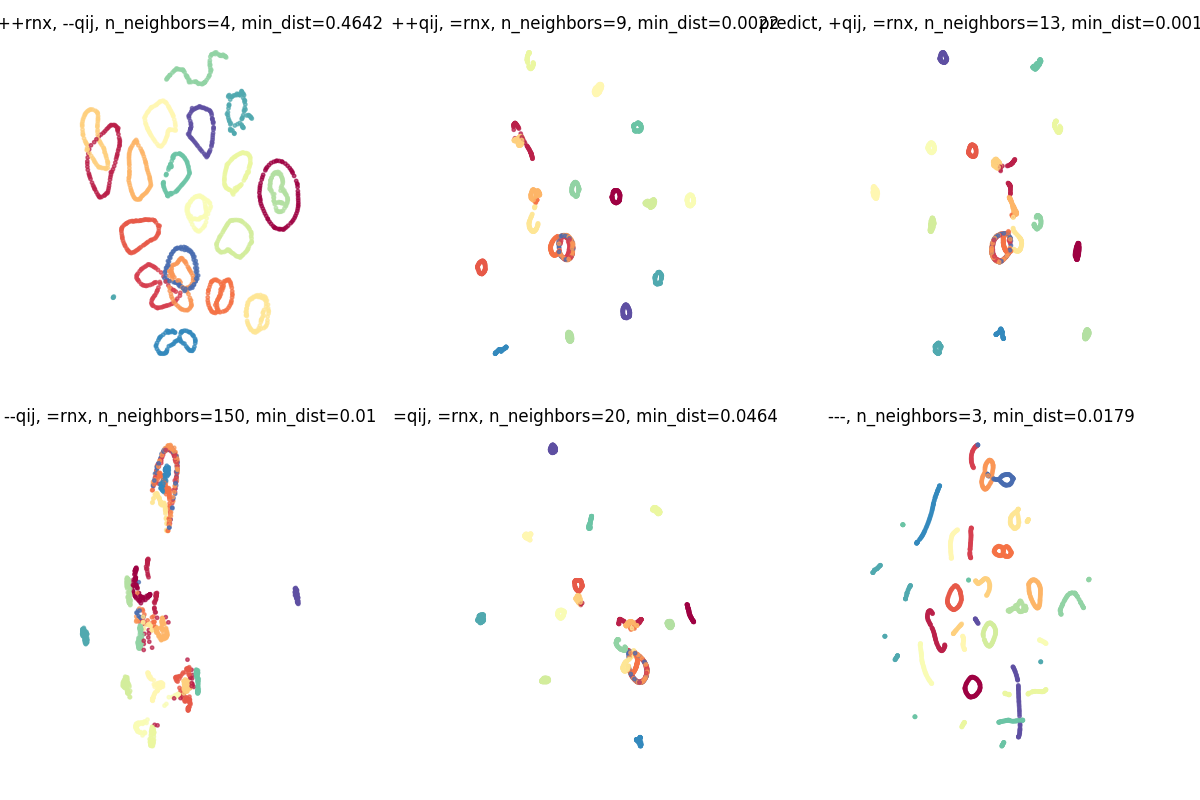
\includegraphics[width=\linewidth]{COIL20_umap_show}
    \end{subfigure}
    \caption{Metamaps and visualizations with hyperparameters by BayOpt based on $f_{score}$ for COIL20.}
    \label{fig:umap:meta:COIL20}
\end{figure*}

%% FIGURE compare 2 scores UMAP
\begin{figure}[ht!]
    \centering
    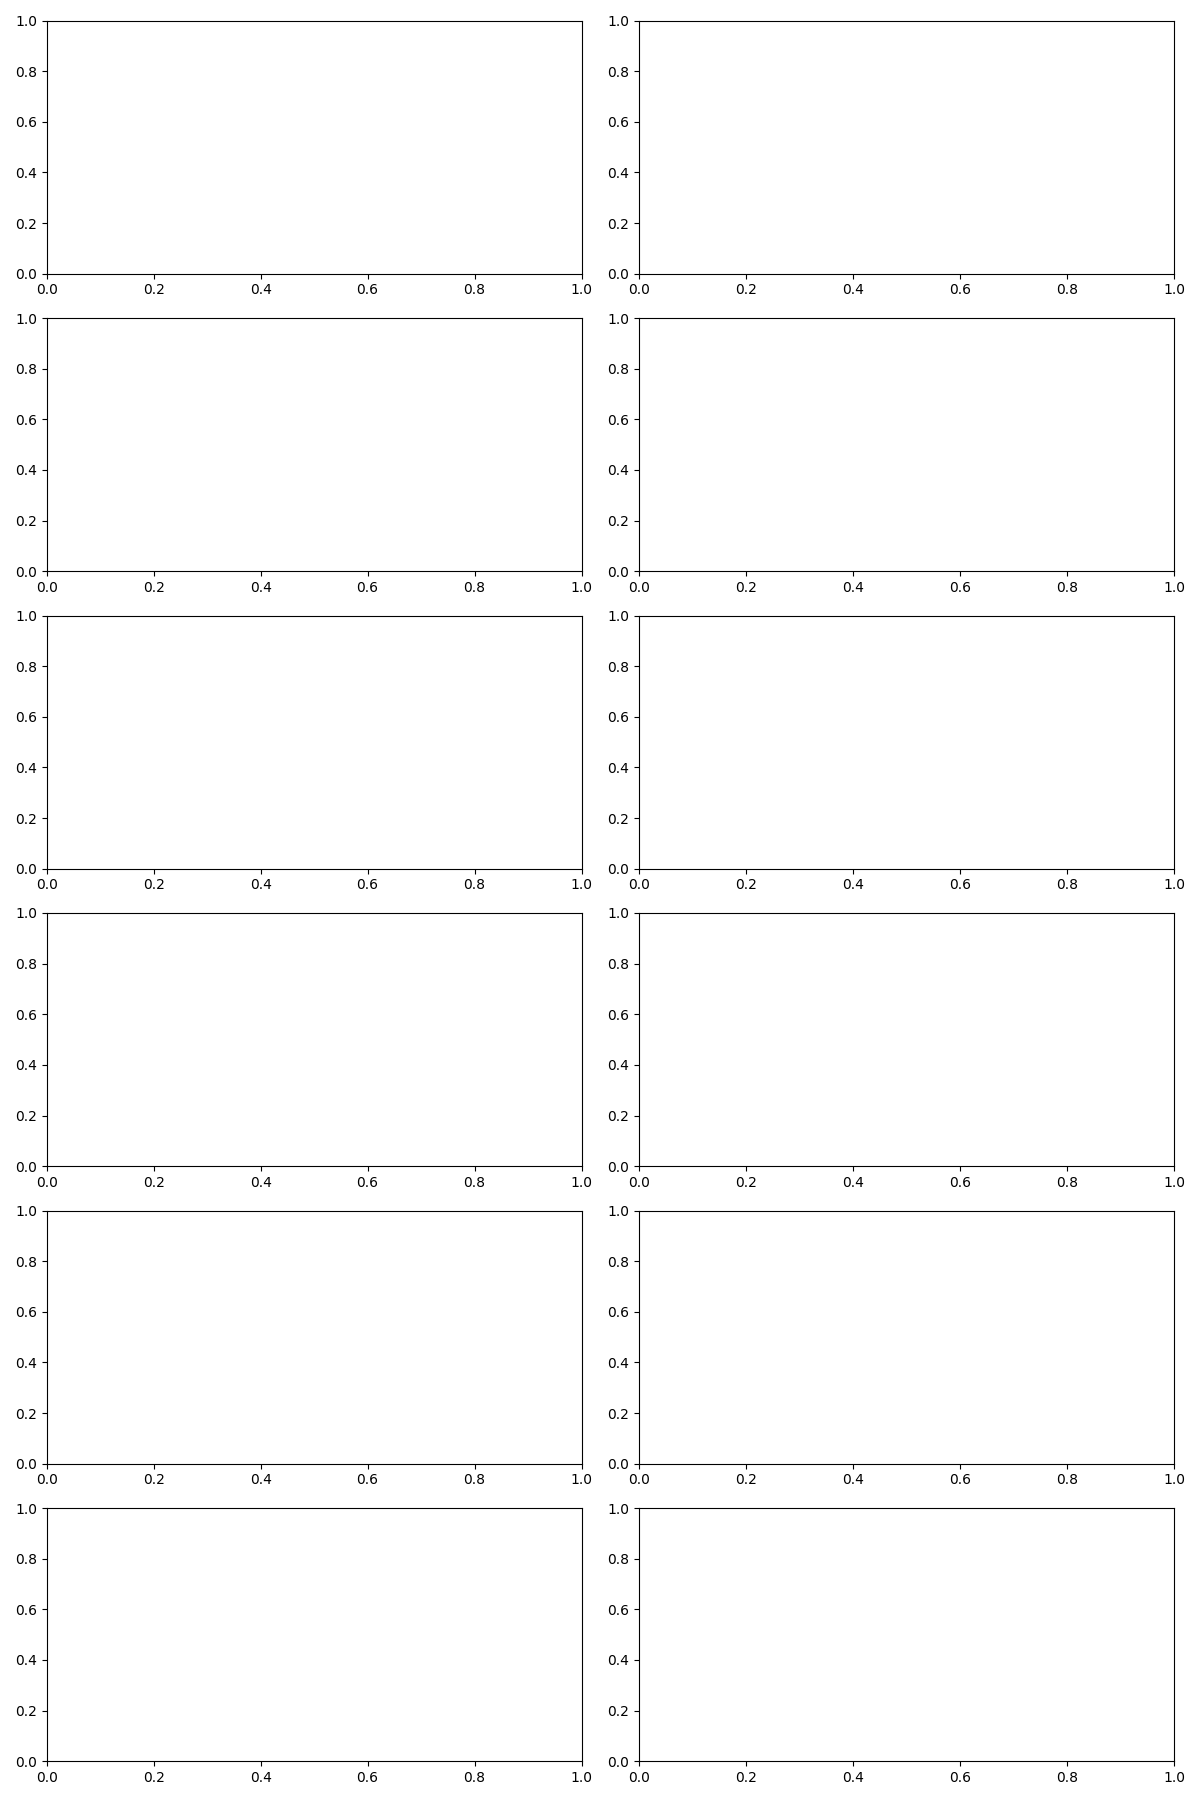
\includegraphics[width=\linewidth]{umap2D_compare}
    \caption{Compare $f_{score}$ and $AUC_{log}RNX$ for UMAP embeddings.}
    \label{fig:score:umap2D:compare}
\end{figure}

As for $t$-SNE in Section~\ref{sec:result:bo:tsne}, metamaps of the different visualizations that can be generated by UMAP are presented at the top of Fig.~\ref{fig:umap:meta:COIL20}, and four different visualizations are selected and shown at the bottom of the figure.
The first visualization (bottom left of Fig.~\ref{fig:umap:meta:COIL20}) presents the visualization generated by UMAP with the best predicted combination of hyperparameter values, according to $f_{score}$.
The next two visualizations are considered good by $AUC_{log}RNX$, but not by $f_{score}$.
In the second visualization, several groups are overlapping. Since the points in same group are not close together, $f_{score}$ is smaller than for the first visualization.
The last visualization belongs to a region of points in the metamaps that have low values for both scores.
These regions are the ones that are never highlighted in the metamaps, which correspond to visualizations that have a too large {n\_neighbors} and/or a too large {min\_dist}. 

%%%%%%%%%%%%%%%%%%%%%%%%%%%%%%%%%%%%%%%%%%%%%%%%%%%%%%%%%%%%%%%%%%%%%%%%%%%%%%%%%%%%%%%%%%%%%%%
\subsection{BayOpt for Hyperparameter Tuning with $f_{score}$}\label{sec:result:bo}
As empirically proved in the previous sections, $f_{score}$ is a reliable score to evaluate the quality of the embeddings.
BayOpt is widely used for hyperparameter tuning, when the target function is well-defined and assures to find global maximum of a well-formed function like $f_{score}$.
In Sec~\ref{sec:result:bo:tsne} and Sec~\ref{sec:result:bo:umap}, $f_{score}$ is evaluated for the tasks of tuning one hyperparameter under BayOpt framework for $t$-SNE two hyperparameters for UMAP, respectively.
% However naive search through the grid of hyperparameters is exponentially expensive when the number of hyperparameters increases.
% BayOpt helps to explore the parameter spaces efficiently and focus the computation only on the zones of potential parameters which give high values for the target function.
% It is widely used for hyperparameter tuning, when the target function is well-defined and assures to find global maximum of a well-formed function like $f_{score}$.
% $AUC_{log}RNX$ score or the BIC-based score can be used as a target function in BayOpt.
% However, our experiments show that $AUC_{log}RNX$ does not always work well with UMAP's embedding, especially in the case of tuning two UMAP's hyperparameters at the same time.
% The BIC-based score, by definition, is tied to $t$-SNE and does not work for other DR methods.
% $f_{score}$ is designed to be independent to the DR methods and to be flexible to the input constraints.
% In this section, the input constraints are generated from 10 labeled points per class for any given dataset.
% $f_{score}$, which is flexible by design, can find the best visualization w.r.t. any set of input constraints.
% This task can not be achieved neither by $AUC_{log}RNX$ nor by BIC-based score.

\subsubsection{BayOpt for Tuning One Parameter of $t$-SNE}\label{sec:result:bo:tsne}

%% FIGURE BO tSNE
\begin{figure}[ht!]
    \begin{subfigure}[b]{.46\linewidth}
        \centering
        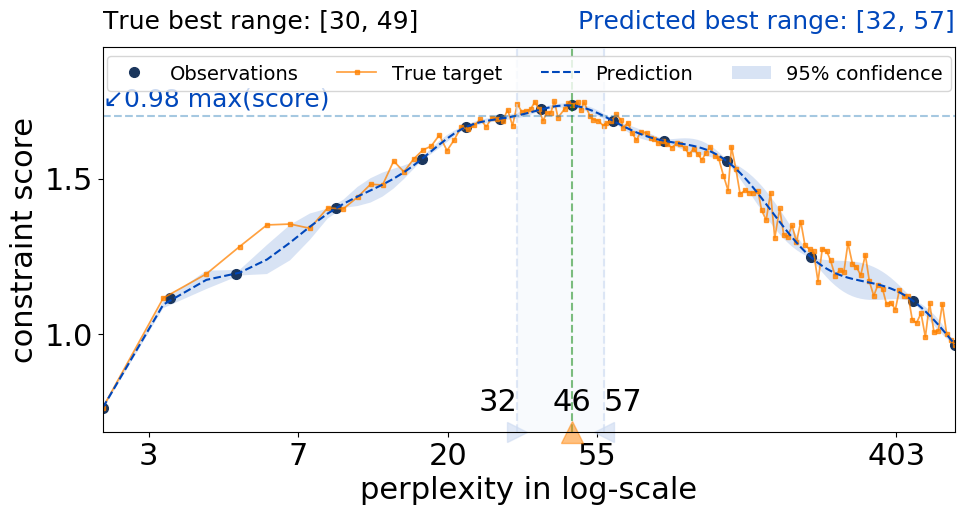
\includegraphics[width=\linewidth]{DIGITS_tsne_bo.png}
        \caption{DIGITS}
    \end{subfigure}
    ~
    \begin{subfigure}[b]{.46\linewidth}
        \centering
        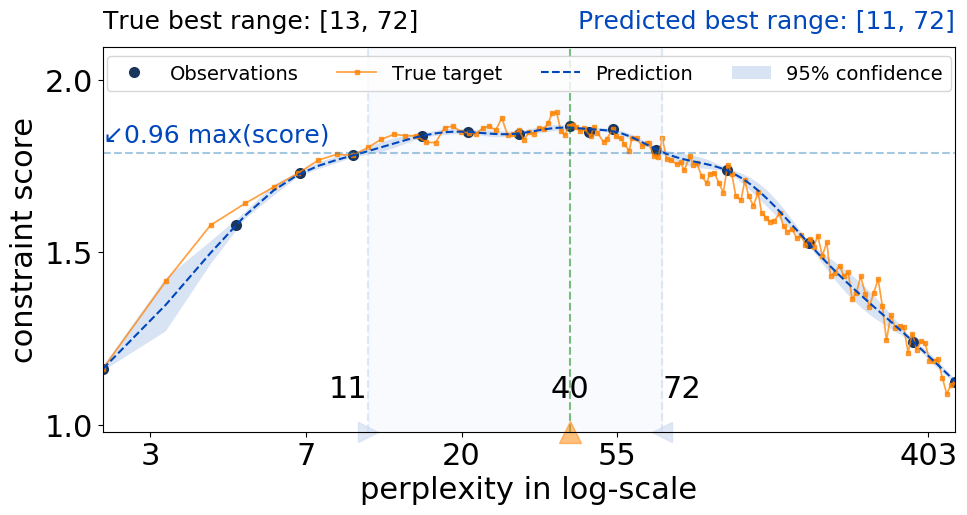
\includegraphics[width=\linewidth]{COIL20_tsne_bo.png}
        \caption{COIL20}
    \end{subfigure}
    \vfill
    \begin{subfigure}[b]{.46\linewidth}
        \centering
        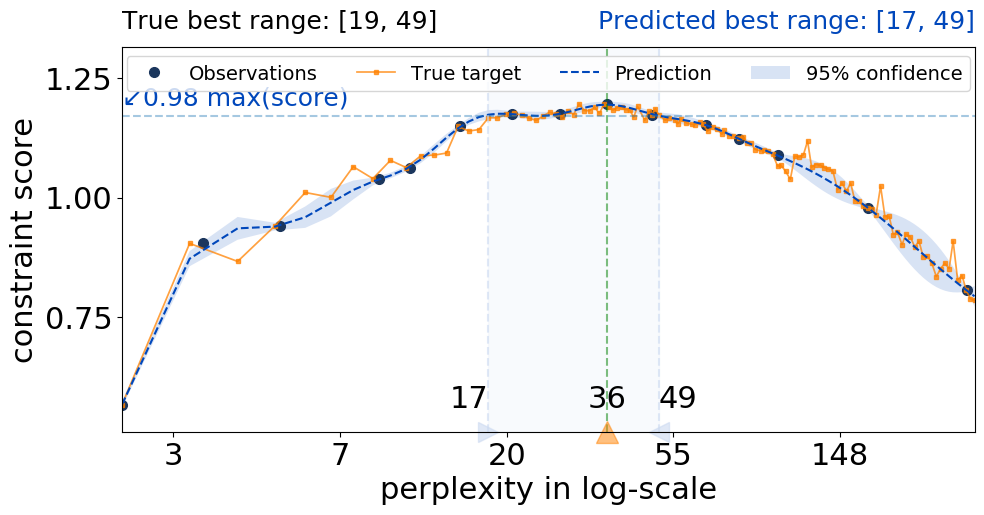
\includegraphics[width=\linewidth]{FASHION1000_tsne_bo.png}
        \caption{{FASHION\_1K}}
    \end{subfigure}
    ~
    \begin{subfigure}[b]{.46\linewidth}
        \centering
        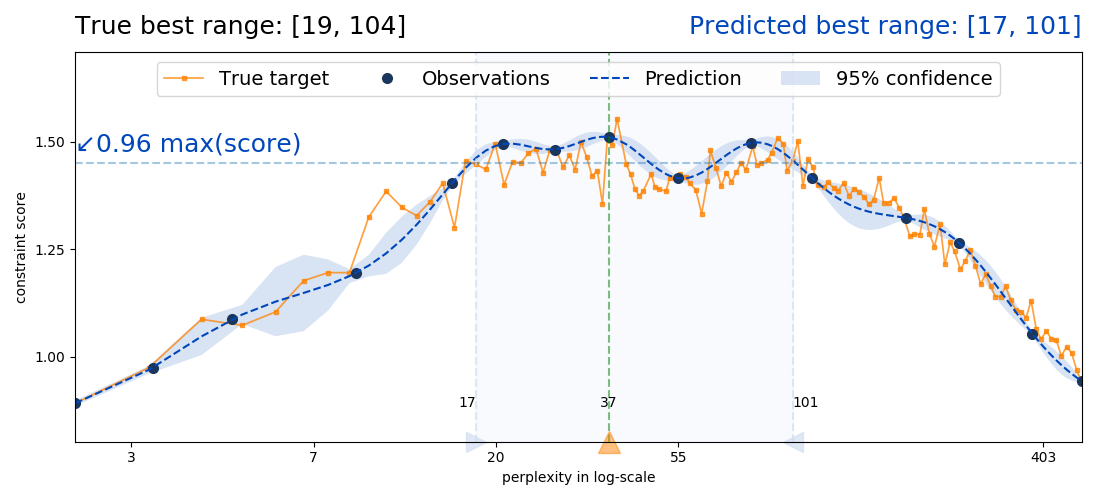
\includegraphics[width=\linewidth]{FASHION_MOBILENET_tsne_bo.png}
        \caption{{FASH\_MOBI}}
    \end{subfigure}
    ~
    \vfill
    \begin{subfigure}[b]{.46\linewidth}
        \centering
        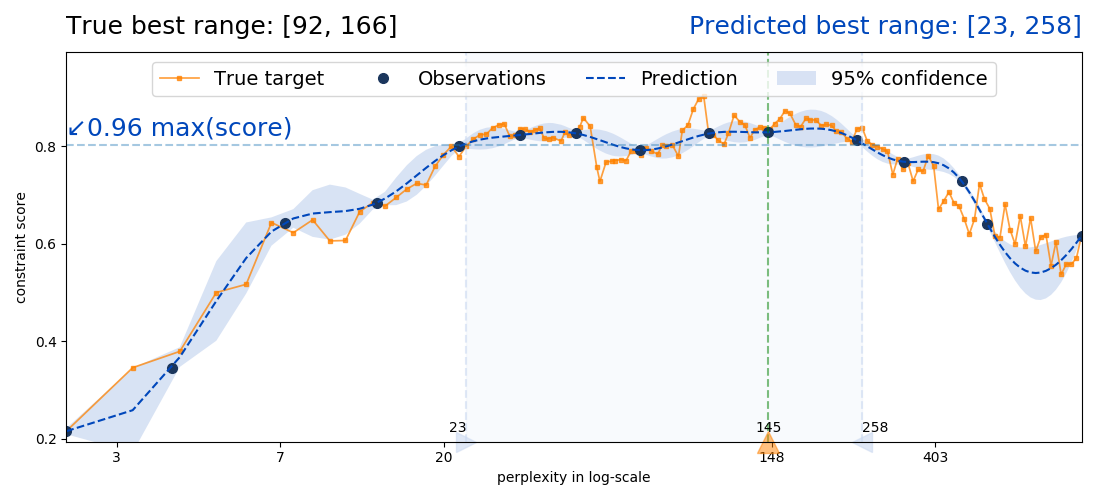
\includegraphics[width=\linewidth]{20NEWS5_tsne_bo.png}
        \caption{5NEWS}
    \end{subfigure}
    ~
    \begin{subfigure}[b]{.46\linewidth}
        \centering
        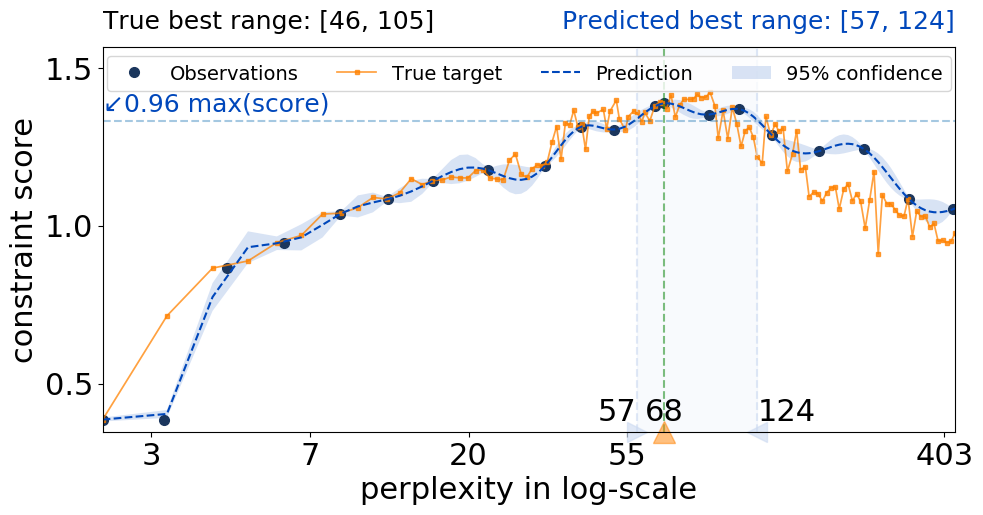
\includegraphics[width=\linewidth]{NEURON_1K_tsne_bo.png}
        \caption{{NEURON\_1K}}
    \end{subfigure}
    \caption{BayOpt approach for  $t$-SNE}
    \label{fig:tsne:bo:all}
\end{figure}

Fig.~\ref{fig:tsne:bo:all} demonstrates how BayOpt works for tuning $t$-SNE's perplexity for all six selected datasets.
% As shown empirically in the previous section, 10 labeled instances for each class suffice for a stable score.
% The scores are calculated for all sampled perplexity values $\in [2, N/3]$, with $N$ being the number of instances in the dataset.
For all datasets of various sizes (from 1000 to around 3000 instances), the scores needs to be evaluated for only 15 selected perplexities.
% These perplexity values are selected by BayOpt iteratively, starting with five perplexities randomly initialized.
% The score for each perplexity $p_i$ is calculated and all pairs $\{p_i, f_{score}(p_i)\}$ are used to train the BayOpt model.
% The next predicted perplexity to evaluate is the most promising value according to the BayOpt model.
% When the new perplexity is evaluated, BayOpt gets the new score value and update its model.
% More detail and visual explanation on how BayOpt works with the proposed score function can be found in \ref{app:bo:explain}.
It should be noted that BayOpt does not approximate the score function, but tries to find its maximum value instead.
% Fig.~\ref{fig:tsne:bo:all} shows the prediction of the best perplexity for BayOpt on each dataset, with a convergence after only 15 iterations.
The best predicted perplexity range (in which the predicted score is superior to 96\% of the maximum predicted score) is highlighted in the vertical region.
BayOpt does not only find the best hyperparameter values, but also indicate the region in which it is not certain about its prediction.
This is usually the region of high perplexity values, where the $f_{score}$ has large distortions.
% [TODO](Minh: move to BO intro section.) Instead of evaluating the score functions for all values of perplexity, BayOpt framework can intelligently choose a limited number of potential perplexities to evaluate and assures to always find a global maximum when it converges.

\subsubsection{BayOpt for Tuning Two Parameters of UMAP}\label{sec:result:bo:umap}

%% FIGURE BO UMAP
\begin{figure}[ht!]
    \begin{subfigure}[b]{.48\linewidth}
        \centering
        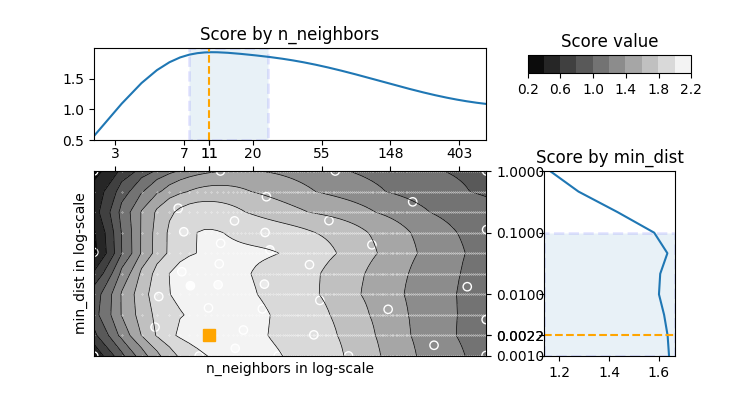
\includegraphics[width=\linewidth]{DIGITS_umap_predicted_score}
        \caption{DIGITS}
        \label{fig:bo:umap:predict:DIGITS}
    \end{subfigure}
    ~
    \begin{subfigure}[b]{.48\linewidth}
        \centering
        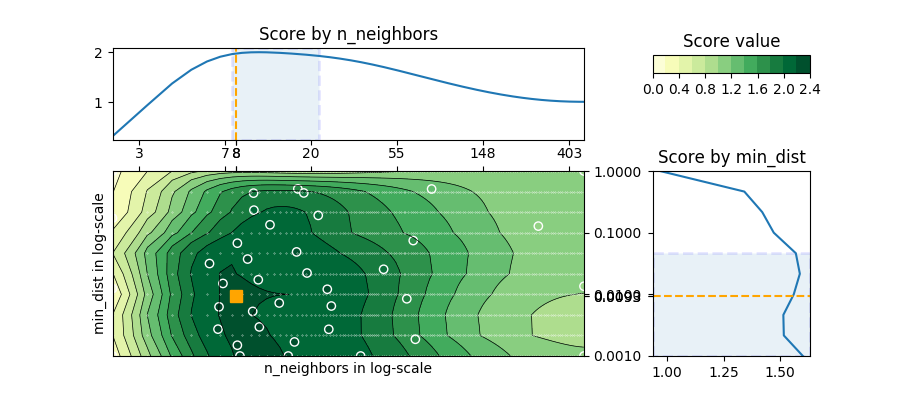
\includegraphics[width=\linewidth]{COIL20_umap_predicted_score}
        \caption{COIL20}
        \label{fig:bo:umap:predict:COIL20}
    \end{subfigure}
    \vfill
    \begin{subfigure}[b]{.48\linewidth}
        \centering
        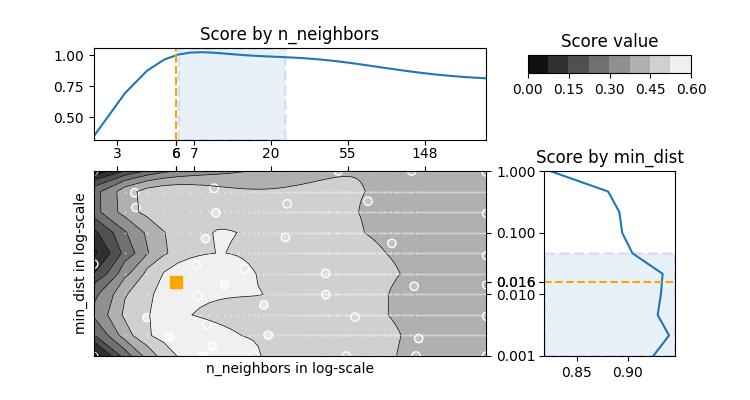
\includegraphics[width=\linewidth]{FASHION1000_umap_predicted_score}
        \caption{{FASHION\_1K}}
        \label{fig:bo:umap:predict:FASHION1K}
    \end{subfigure}
    ~
    \begin{subfigure}[b]{.48\linewidth}
        \centering
        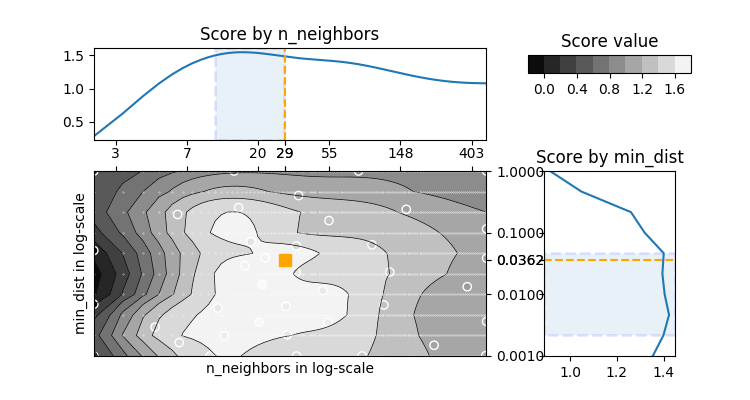
\includegraphics[width=\linewidth]{FASHION_MOBILENET_umap_predicted_score}
        \caption{{FASH\_MOBI}}
        \label{fig:bo:umap:predict:FASHMOBI}
    \end{subfigure}
    \vfill
    \begin{subfigure}[b]{.48\linewidth}
        \centering
        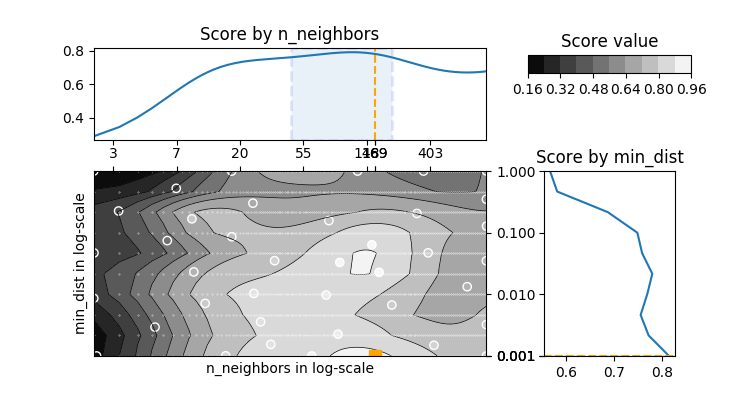
\includegraphics[width=\linewidth]{20NEWS5_umap_predicted_score}
        \caption{5NEWS}
        \label{fig:bo:umap:predict:5NEWS}
    \end{subfigure}
    ~
    \begin{subfigure}[b]{.48\linewidth}
        \centering
        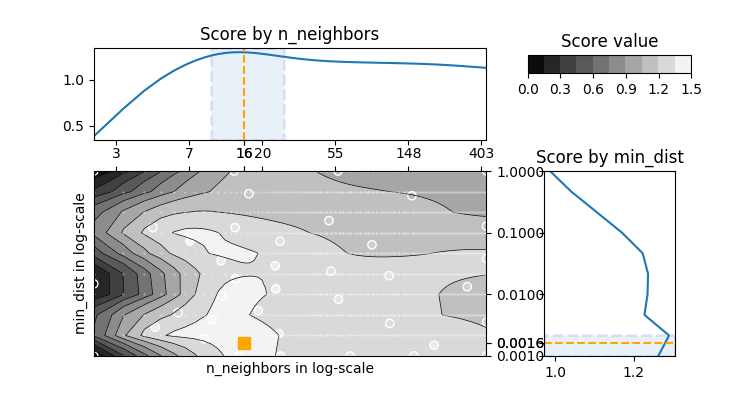
\includegraphics[width=\linewidth]{NEURON_1K_umap_predicted_score}
        \caption{{NEURON\_1K}}
        \label{fig:bo:umap:predict:NEURON1K}
    \end{subfigure}
    \caption{BayOpt for tuning the two hyperparameters of UMAP for all datasets.}
    \label{fig:bo:umap:predict}
\end{figure}

Instead of evaluating thousands of combinations of two hyperparameters of UMAP, BayOpt converges only after 40 iterations for all six experimented datasets.


% In this section, we show that using BayOpt with an $f_{score}$ evaluating a two-hyperparameters DR also results in picking quality visualizations. In order to show that, UMAP hyperparameters are tuned.
% The first UMAP hyperparameter, {n\_neighbors}, plays the same role as the perplexity of $t$-SNE and LargeVis, which controls how large structures in the data should be conserved.
% {n\_neighbors} affects the construction of the k-neighbor graph in HD.
% A small value leads to many small connected components in the visualization, while a large value provides a boarder view of the data.
% A suggested range for {n\_neighbors} is $[5, 50]$.

% The second UMAP hyperparameter, {min\_dist}, affects directly the output since it controls how tightly points are packed together. It is considered to be most important hyperparameter for UMAP \cite{mcinnes2018umap}.
% The recommended range for {min\_dist} is $[0.001, 0.5]$.

% Finding the best combination of these two hyperparameters for a specified dataset is hard.
% A naive approach requires thousands of evaluations.
% $f_{score}$ and $AUC_{log}RNX$ are evaluated for all UMAP embeddings, based on a grid of around 150 values for {n\_neighbors} $\in [2, N/3]$ (depending on the size of the dataset), and 10 values for {min\_dist} $\in [0.001, 1]$ in logarithmic scale.

% \begin{figure}%[pos=h]
%     \begin{subfigure}[b]{.76\linewidth}
%         \centering
%         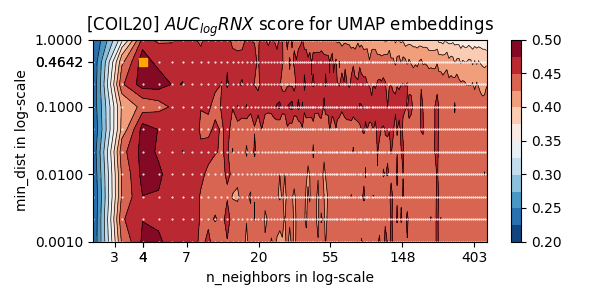
\includegraphics[width=\textwidth]{COIL20_umap_auc_rnx}
%         \caption{$AUC_{log}RNX$ score.}
%         \label{fig:bo:umap:COIL20:rnx}
%     \end{subfigure}
%     ~
%     \begin{subfigure}[b]{.76\linewidth}
%         \centering
%         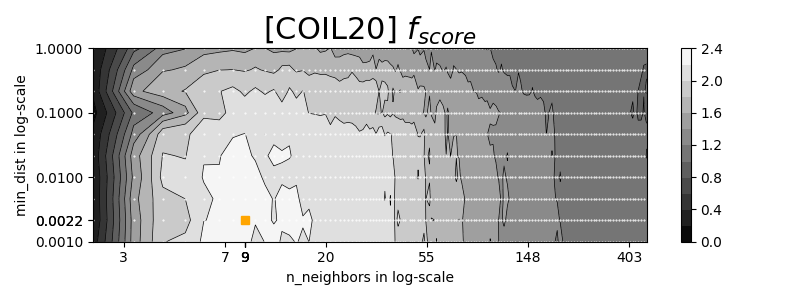
\includegraphics[width=\textwidth]{COIL20_umap_qij_score}
%         \caption{$f_{score}$}
%         \label{fig:bo:umap:COIL20:fscore}
%     \end{subfigure}
%     ~
%     \begin{subfigure}[b]{.98\linewidth}
%         \centering
%         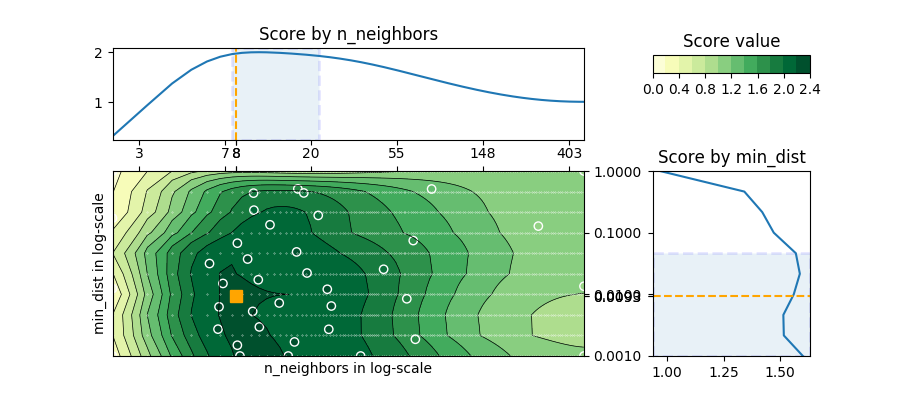
\includegraphics[width=\textwidth]{COIL20_umap_predicted_score}
%         \caption{BayOpt predicted score}
%         \label{fig:bo:umap:COIL20:prediction}
%     \end{subfigure}
%     ~
%     \caption{BayOpt for tuning the two hyperparameters of UMAP for COIL20.}
%     \label{fig:bo:umap:COIL20}
% \end{figure}

Fig.~\ref{fig:bo:umap:COIL20:rnx} and Fig.~\ref{fig:bo:umap:COIL20:fscore} show $AUC_{log}RNX$ and $f_{score}$ for every combination of hyperparameters for COIL20.
% $AUC_{log}RNX$ cannot investigates the relevant of the two hyperparameters, as indicated by the homogeneous zones on the left and on top of Fig.~\ref{fig:bo:umap:COIL20:rnx}.
% Indeed, when {n\_neighbors} is small (between 3 and 8), {min\_dist} does not have strong affect. And when {min\_dist} is large enough (larger than 0.1), {n\_neighbors} does not have strong affect either.
As it can be observed in Fig.~\ref{fig:bo:umap:COIL20:fscore}, $f_{score}$ can identify a small zone of good combinations, which makes the hyperparameter tuning task easier and more reliable. The prediction of the best visualization by BayOpt based on $f_{score}$ is presented in Fig.~\ref{fig:bo:umap:COIL20:prediction}.
With BayOpt, only 40 combinations are selected and evaluated to find the best visualization, instead of evaluating thousands of combinations.


%%%%%%%%%%%%%%%%%%%%%%%%%%%%%%%%%%%%%%%%%%%%%%%%%%%%%%%%%%%%%%%%%%%%%%%%%%%%%%%%%%%%%%%%%%%%%%%
%%%%%%%%%%%%%%%%%%%%%%%%%%%%%%%%%%%%%%%%%%%%%%%%%%%%%%%%%%%%%%%%%%%%%%%%%%%%%%%%%%%%%%%%%%%%%%%
\subsection{Flexibility of $f_{score}$}\label{sec:result:flexibility}

%% FIGURE Score flexibility
\begin{figure*}[ht!]
    \centering
    \begin{subfigure}[b]{.32\linewidth}
        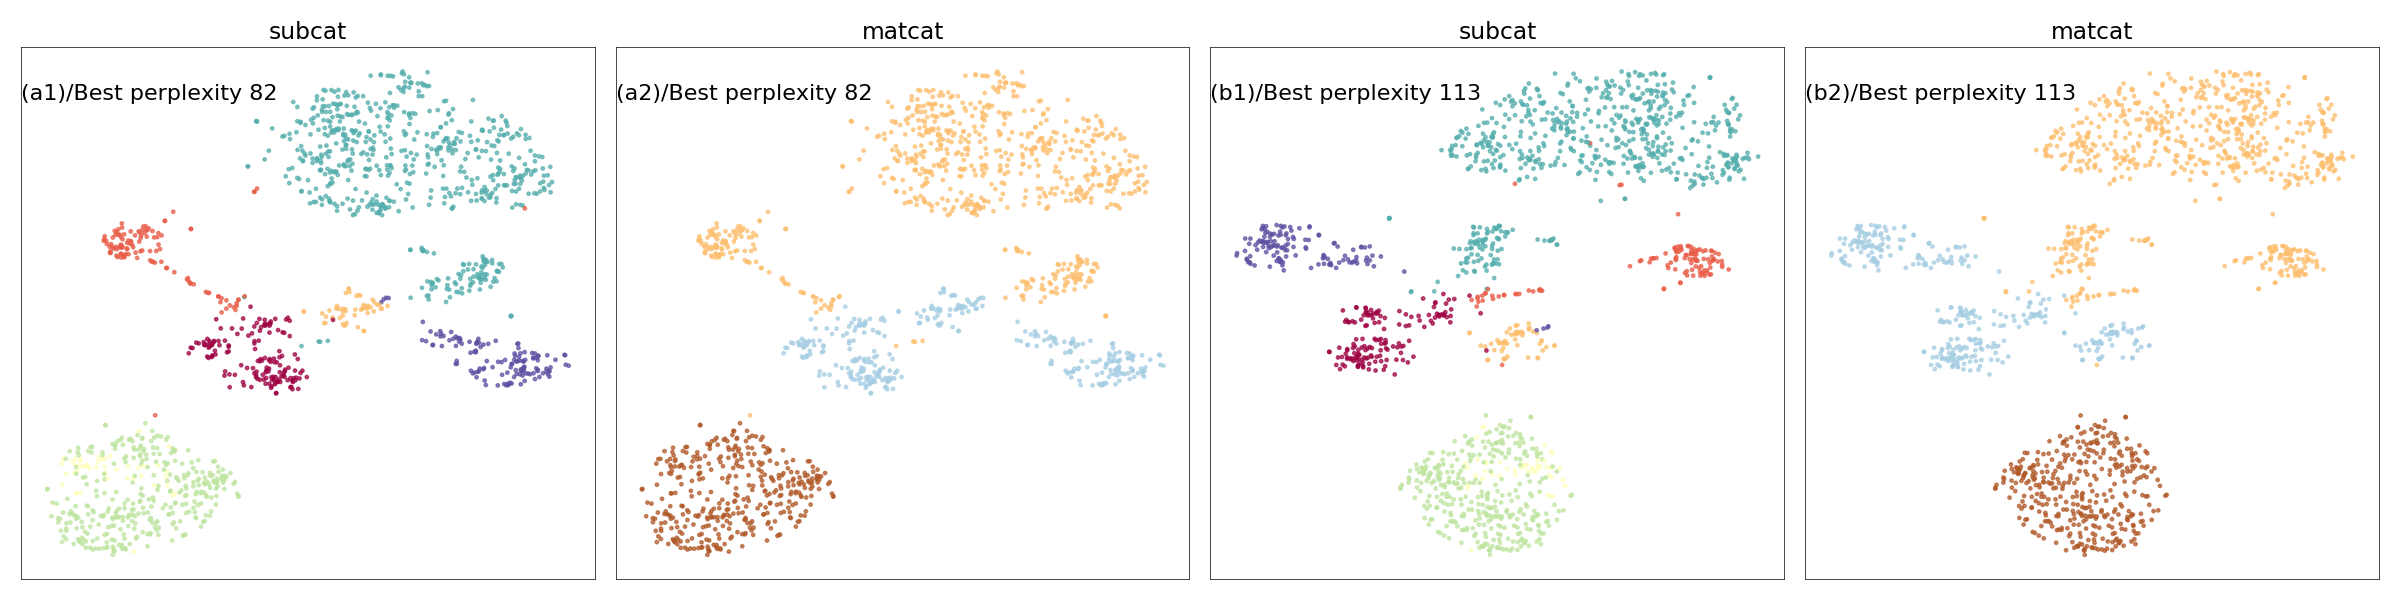
\includegraphics[width=\linewidth]{FASHION_MOBILENET_score_flexibility}
        \caption{{FASH\_MOBI} dataset}
        \label{fig:flexibility:FASHMOBI}
    \end{subfigure}
    ~
    \begin{subfigure}[b]{.32\linewidth}
        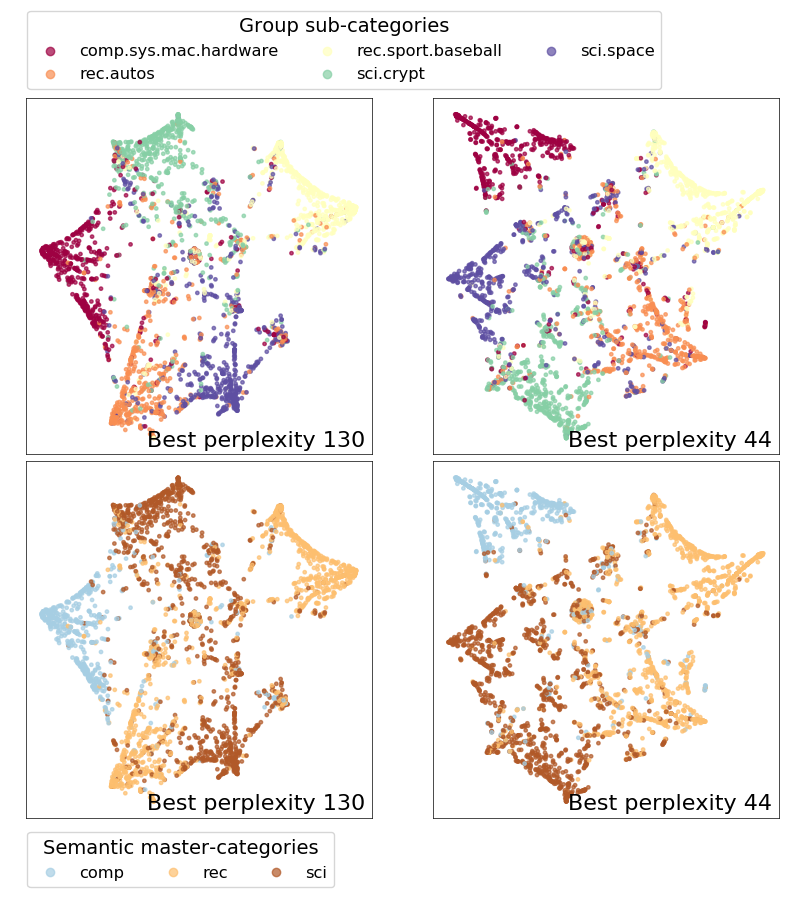
\includegraphics[width=\linewidth]{20NEWS5_score_flexibility}
        \caption{5NEWS dataset}
        \label{fig:flexibility:5NEWS}
    \end{subfigure}
    ~
    \begin{subfigure}[b]{.32\linewidth}
        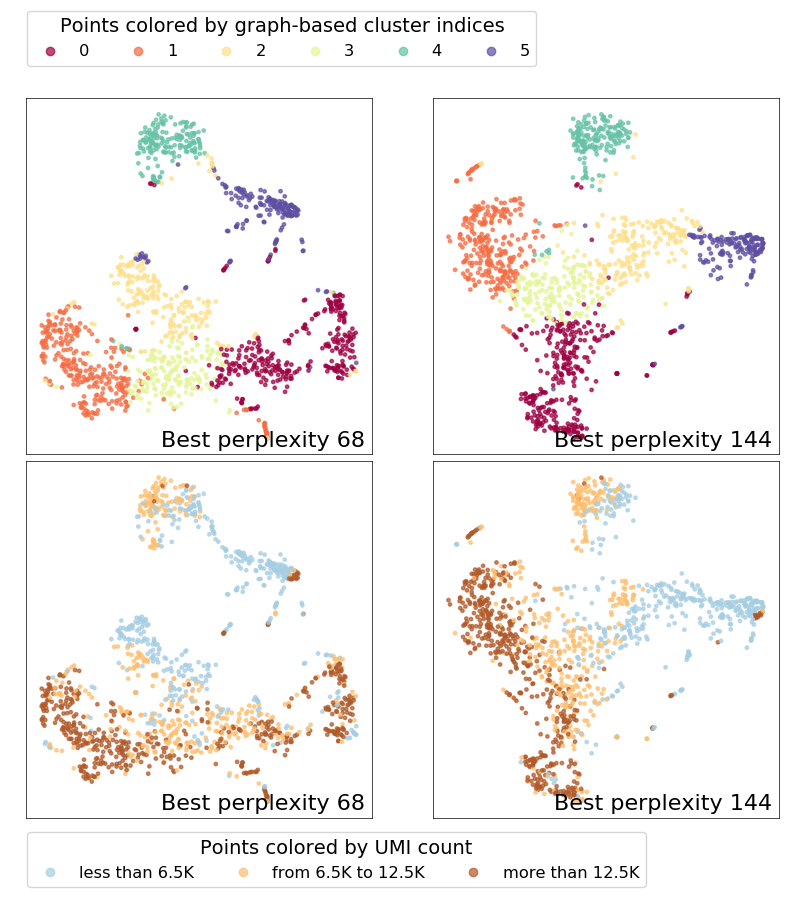
\includegraphics[width=\linewidth]{NEURON_1K_score_flexibility}
        \caption{{NEURON\_1K} dataset}
        \label{fig:flexibility:NEURON1K}
    \end{subfigure}
    ~
    \caption{Flexibility of $f_{score}$.}
    \label{fig:flexibility}
\end{figure*}

The visualization quality metrics presented in Section~\ref{subsec:qual_metrics_background} take a given embedding as input and produce a measurement.
For instance, $AUC_{log}RNX$ measures how well the neighborhood information is preserved and the BIC-base score measures the trade-off between the KL loss of $t$-SNE and the perplexity.
These score calculated by these metrics are deterministic since the characteristics measured by them are fixed.
In contrast, $f_{score}$, while also deterministic, is a function of given constraints that evaluates how well these constraints are preserved.
$f_{score}$ can measure the embeddings differently, depending on the relation encoded in the given input constraints. The quality measurement of $f_{score}$ is therefore flexible w.r.t. to the user needs.

In the previous experiments, the constraints generated from class labels reflected naturally the class-relationship between the instances.
However, if the users want to see different pattern in the data, they can specify different constraints in $f_{score}$ to describe what they need.

Concrete examples with $t$-SNE embeddings for three real world datasets are presented in this section.
The first example is provided for {FASH\_MOBI} with seven sub-groups: 'Bags', 'Bottomwear', 'Jewellery', 'Sandal', 'Shoes', 'Topwear' and 'Watches'.
Given 10 labeled points for each sub-groups, BayOpt finds 82 as the perplexity for $t$-SNE embedding that best respect the constraints.
As shown in the top-left plot of Fig~\ref{fig:flexibility:FASHMOBI}, the chosen visualization presents the seven sub-groups as well detached.
A hierarchical grouping can also be used. This means that 'Bag', 'Jewellery', 'Watches' are grouped as 'Accessories', 'Sandal', 'Shoes' are grouped into 'Footware' and 'Topwear', 'Bottomware' are grouped into 'Apparel'.
The previously-chosen perplexity of 82 fits well the seven sub-groups, but does not reveal these three hierarchical groups in the visualization.
For constraints generated based on these hierarchical groups, BayOpt used with $f_{score}$ provides a new best perplexity of 113, which better reveal the structure of the hierarchical groups, as it can be observed in the bottom-right corner of Fig~\ref{fig:flexibility:FASHMOBI}.

The second example concerns semantic labels for the textual 5NEWS dataset.
The five original classes can be regrouped into three more general topics, e.g. 'rec.autos', 'rec.sport.baseball' into a group of sportive records 'rec', and 'sci.space', 'sci.crypt' into a scientific group 'sci'. The bottom-left visualization in Fig.~\ref{fig:flexibility:5NEWS} is a good visualization for the 5 classical labels, but do not separate the three new general topics. When optimizing $f_{score}$ with constraints based on the three more general topics, the bottom-right visualization in Fig.~\ref{fig:flexibility:5NEWS} is provided. It can be observed that this new visualization better separate the new categories that we want to analyze.

The last example is for the genetic dataset NEURON\_1K.
The original 1301 cells are grouped into 6 classes found by a graph-based clustering algorithm.
These classes are characterized by the transcriptome profiles of individual cells (presented in the RNA sequences).
However, another important aspect to characterize individual cells is the count of absolute numbers of molecules: the unique molecular identifier (UMI)~\cite{kivioja2011counting}. 
The cells are regrouped into three new groups: having less than 6.5K molecules, having from 6.5K to 12.5K molecules and having more than 12.5K molecules.
Fig.~\ref{fig:flexibility:NEURON1K} illustrates the new visualization found by $f_{score}$ with the new constraints.
It should be noted that this optimal perplexity w.r.t. the \emph{UMI count} is never discovered by neither $AUC_{log}RNX$, nor the BIC-based score.

%%%%%%%%%%%%%%%%%%%%%%%%%%%%%%%%%%%%%%%%%%%%%%%%%%%%%%%%%%%%%%%%%%%%%%%%%%%%%%%%%%%%%%%%%%%%%%%
%%%%%%%%%%%%%%%%%%%%%%%%%%%%%%%%%%%%%%%%%%%%%%%%%%%%%%%%%%%%%%%%%%%%%%%%%%%%%%%%%%%%%%%%%%%%%%%
\section{Discussion}\label{sec:discussion}

$t$-SNE, LargeVis and UMAP are widely used since they produce good visualizations.
Their objective is to preserve the neighborhood information, at the cost of loosing the overall structure of data.
Because of that, several solutions exist in which, for equally good visualizations, some of them highlight a specific view of the overall structure.
It has been shown in our experiments that such a specific, desired structure may exist in the solution space, but like $AUC_{log}RNX$ or the BIC-based score would only reveal one of the global structure view, which may not be the desired one.
$f_{score}$, in addition to be a reliable method to tune DR hyperparameters, is also a flexible score that can reveal a specific, desired desired global structure by users.

This section proposes a discussion on three important topics. First, a discussion on the specific use of BayOpt for optimizing $f_{score}$ is proposed. Second, we discuss the flexibility of the proposed score. Then third, the computational cost of $f_{score}$ is studied and discussed, as additional inputs have to be provided to compute the score, i.e. the constraints.

\subsection{Why using BayOpt for $f_{score}$?}
The proposed $f_{score}$ has an advantage in its flexibility, but the score value is not deterministic.
With the same number of labeled instances or the same number of constraints, the score may vary w.r.t. chosen sets of constraint pairs.
The BayOpt approach fits well in this situation, since it can learn from noisy observation.
The underlying predictive model of the BayOpt framework is a Gaussian process (GP) model.
In the context of our work, the GP model is based on the assumption that similar hyperparameter values give similar embeddings, and thus similar output score values.
In practice, we found that this assumption is true for all three selected DR methods and all experimented datasets (see the curves in Fig.~\ref{fig:score:stability:COIL20} and the contour plots in Fig.~\ref{fig:bo:umap:COIL20}).
In our problem, there is a major reason why the prediction of BayOpt converges quickly to the global optimum (after 15 iterations for tuning $t$-SNE's perplexity and 40 iterations for tuning UMAP's two hyperparameters): the proposed score function is well-formed, which makes it very simple to find its maximum.
% Second, the exploitation strategy used in BayOpt's Expected Improvement acquisition function, combining with the parameters sampled in log-scale helps us quickly discover the good range of parameters and eliminate the range of too small or too large values. (See the density of evaluated points in Fig~\ref{fig:tsne:bo:all} and Fig~\ref{fig:bo:umap:COIL20:prediction}).
Moreover, the iterative predictions of BayOpt are visible (as shown in \ref{app:bo:explain}), which makes the optimization explainable for non-expert users.
Indeed, BayOpt can be run iteratively to investigate why a particular hyperparameter value is chosen, or to directly guide the optimization process. For instance, the user can specify the hyperparameter to evaluate and the GP model will update itself to learn from both the already evaluated $f_{score}$ and the new probed observation.

\subsection{$f_{score}$ is a Flexible Function}
Unlike $AUC_{log}RNX$ or the BIC-based score, which do not depend on external input data, $f_{score}$ is a function of a given ensemble of similar-link constraints $\mathcal{S}$ and dissimilar-link constraints $\mathcal{D}$.
$AUC_{log}RNX$ objectively measures how neighborhoods are preserved without taking into account the prior knowledge of users.
As demonstrated in Sec.~\ref{sec:result:flexibility} with three real world datasets, $f_{score}$ can discover solutions satisfying users' constraints that are never selected by $AUC_{log}RNX$, nor the BIC-based score.
Moreover, the constraint score function can be easily modified to adapt to different criteria, such as the contrastive measure or the triplet measure.
These are adapted version based on the idea of contrastive loss~\cite{logeswaran2018efficient} and triplet loss~\cite{schroff2015facenet}, which use several selected anchor points, their positive examples (connected by similar-links) and their negative examples (connected by dissimilar-links).
% $\mathbb{E}_{y, y_+, y_-} \Big[ -\log \Big( \frac{exp(y^T y_+)}{exp(y^T y_+) + exp(y^T y_-)} \Big) \Big]$
% $\mathbb{E}_{y, y_+, y_-} \Big[ max(0, ||y-y_+||^2 - ||y-y_-||^2  \Big]$

\subsection{Computational Efficiency of $f_{score}$}
In practice, dozen labels for each class is enough to find the desired global structure in the data.
$f_{score}$ has a complexity of $O(N^2)$ since it only requires access to the embedding.
Furthermore, the summation over all input pairwise constraints is trivial and efficiently vectorized.
In contrast, $AUC_{log}RNX$ measures how the neighborhood information in HD is preserved in LD, and thus must access to both HD data and the embedding.
It has a high complexity of $O(DN^2logN)$ ($D$ is the dimension of the original data, often be large for image data; and $N$ is the number of data points in a dataset) and may not be applicable for large dataset.
The BIC-based score, despite its simplicity, can only be used for $t$-SNE.
It is designed as a modified cost function of $t$-SNE, with a regularization term to penalize too large perplexities.
The proposed constraint preserving score, $f_{score}$, is computationally more efficient than $AUC_{log}RNX$ and is agnostic w.r.t. the DR method used.

%%%%%%%%%%%%%%%%%%%%%%%%%%%%%%%%%%%%%%%%%%%%%%%%%%%%%%%%%%%%%%%%%%%%%%%%%%%%%%%%%%%%%%%%%%%%%%%
%%%%%%%%%%%%%%%%%%%%%%%%%%%%%%%%%%%%%%%%%%%%%%%%%%%%%%%%%%%%%%%%%%%%%%%%%%%%%%%%%%%%%%%%%%%%%%%
\section{Conclusion and Future Work}\label{sec:conclusion}
The principle contribution of this work is to propose a flexible constraint preserving score to quantitative measure the quality of any DR methods.
This score is used in a Bayesian Optimization framework to find the best visualization of $t$-SNE, LargeVis and UMAP.


\par (1) Repeat the problem of hyperparameter tuning for DR methods and our solution:

+ The proposed constraint-based score is independent to how the embedding is produced and can be used with any DR methods.
This score is built upon a limited number of constraints but can distinguish the visualizations preferring local structure and those preferring global structure.

+ A finding that Bayesian Optimization approach fits well in our problem.


\vspace{8pt}
\par (2) Summary the advantages of the two above elements

+ The constraint-based score agree the the well-known quality metric.

+ This score can be visually represented to explain the violated pairs.

+ By combining this score with BayOpt approach, we can tune many hyperparameters at the same time for many widely used DR methods like $t$-SNE or UMAP.

+ BayOpt takes into account the uncertainty in the score values and also explainable. We can observe the internal optimization step to answer the question: why to choose the next promising hyperparameters to try?

The hyperparameters of $t$-SNE and UMAP make these methods difficult to use correctly but also make them flexible.
These methods can produce different visualizations and reveal different hidden structures in the data.
To evaluate the embedding quality of such flexible methods, we need a flexible score.
The state of the art $AUC_{log}RNX$ metric or the BIC-based score has no flexibility to capture different visualization results.

Future work:

(a) User experiment:
\subsubsection*{The constraint generation can be guided by the users and the visualization quality can be evaluated by them.}
Since the proposed constraint score proved to be stable w.r.t the number of labeled points,
we can use the user-defined labeled points to generate the pairwise constraints.
As demonstrated with the labeled points of three different groups characterized by UMI count in \emph{NEURAL\_1K} dataset, the users can define their need about the structure they look for.
A potential future work is to let the users evaluate qualitatively the quality of the visualization and their satisfaction.

+ Integrate the user's feedback in two stages of our workflow.
The users can select the pairwise constraints or label some points (used to generate the constraints) to build the score.
They can also manually select the next hyperparameters to evaluate in a customized interactive BayOpt framework.

+ Take the preference of the users on the presented visualizations to evaluate the quality of the visualization. We search for if the best visualization selected by the user corresponds to the result of our method.

% \section{Quality metrics}\label{appendix:qual_metrics}

% \section{Stability of $f_{score}$}\label{app:score:stability}

% \section{Metamap and samples for $t$-SNE's embeddings with DIGITS and {FASHION\_1K} datasets}\ref{app:tsne:meta}

% \section{Compare $f_{score}$ with $AUC_{log}RNX$ (default min\_dist 0.1)}\label{app:score:umap:compare}

% \section{Constraint-based Score as Target Function in Bayesian Optimization Approach}\label{app:bo:explain}